%--------------------------------------------------------------------%
%
% Berkas utama templat LaTeX.
%
% author Petra Barus, Peb Ruswono Aryan, Faris Rizki Ekananda
%
%--------------------------------------------------------------------%
%
% Berkas ini berisi struktur utama dokumen LaTeX yang akan dibuat.
%
%--------------------------------------------------------------------%

\documentclass[bahasa, 12pt, a4paper, onecolumn, oneside, final]{report}

%-------------------------------------------------------------------%
%
% Konfigurasi dokumen LaTeX untuk laporan tesis IF ITB
%
% @author Petra Novandi
%
%-------------------------------------------------------------------%
%
% Berkas asli berasal dari Steven Lolong
%
%-------------------------------------------------------------------%

% Ukuran kertas
\special{papersize=210mm,297mm}

% Setting margin
\usepackage[top=3cm,bottom=3cm,left=4cm,right=3cm]{geometry}

\usepackage{mathptmx}

% Judul bahasa Indonesia
\usepackage[bahasa]{babel}

% Format citation
\usepackage[style=apa,backend=biber]{biblatex}

\usepackage[utf8]{inputenc}
\usepackage{graphicx}
\usepackage{titling}
\usepackage{blindtext}
\usepackage{sectsty}
\usepackage{chngcntr}
\usepackage{etoolbox}
\usepackage{hyperref}       % Package untuk link di daftar isi. Ubah jadi \usepackage[hidelinks]{hyperref} apabila ingin menghilangkan kotak merah disekitar link
\usepackage{titlesec}       % Package Format judul
\usepackage{titletoc}       % Package Format judul di toc
\usepackage{tocbibind}      % Package untuk masukkan toc, lot, lof ke Daftar Isi
\usepackage{scrwfile}       % Package untuk membuat Daftar Lampiran dari toc
\usepackage{parskip}
\usepackage{afterpage}
\usepackage{relsize}
\usepackage{listings}       % Package lstlistings and stuff
\usepackage{xcolor}

\graphicspath{{resources/}}   % letak direktori penyimpanan gambar

% Setting daftar lampiran
\newcommand*{\lopname}{DAFTAR LAMPIRAN}
\TOCclone[\lopname]{toc}{atoc}
\addtocontents{atoc}{\protect\value{tocdepth}=-1}
\newcommand\listofappendices{
  \cleardoublepage
  \phantomsection
  \listofatoc
  \addcontentsline{toc}{chapter}{\lopname}
}

\newcommand*\savedtocdepth{}
\AtBeginDocument{%
  \edef\savedtocdepth{\the\value{tocdepth}}%
}

\let\originalappendix\appendix
\renewcommand\appendix{%
  \originalappendix
  \cleardoublepage
  \addtocontents{toc}{\protect\value{tocdepth}=-1}%
  \addtocontents{atoc}{\protect\value{tocdepth}=\savedtocdepth}%

  \titlecontents{chapter}
    [0pt]
    {\bfseries}
    {Lampiran \thecontentslabel.\quad}
    {}
    {\hfill\contentspage}

  \titleformat{\chapter}[block]
    {\bfseries}
    {\chaptertitlename\ \thechapter.\quad}{0pt}
    {\bfseries}
}

% Define colors
\colorlet{punct}{red!60!black}
\definecolor{delim}{RGB}{20,105,176}
\colorlet{numb}{magenta!60!black}
\definecolor{eclipseStrings}{RGB}{42,0.0,255}
\definecolor{eclipseKeywords}{RGB}{127,0,85}

% Hilangkan titik pada toc
\makeatletter
\renewcommand{\@dotsep}{10000} 
\makeatother

% Setel title pada chapter-chapter di toc, lof, lot
\titlecontents{chapter}
  [0pt]
  {\bfseries}
  {\MakeUppercase{Bab} \thecontentslabel\quad\uppercase}
  {}
  {\hfill\contentspage}
\titlecontents{figure}
  [0pt]
  {}
  {Gambar \thecontentslabel.\quad}
  {}
  {\hfill\contentspage}
\titlecontents{table}
  [0pt]
  {}
  {Tabel \thecontentslabel.\quad}
  {}
  {\hfill\contentspage}

% Masukin Daftar Pustaka ke toc
\let\originalprintbibliography\printbibliography
\renewcommand\printbibliography{%
  \phantomsection
  \cleardoublepage
  \originalprintbibliography
  \addcontentsline{toc}{chapter}{\bibname}
}

% Line satu setengah spasi
\renewcommand{\baselinestretch}{1.5}

% Setting judul
\chapterfont{\centering \Large}
\titleformat{\chapter}[display]
  {\Large\centering\bfseries}
  {\chaptertitlename\ \thechapter}{0pt}
    {\Large\bfseries\uppercase}

% Setting nomor pada subbsubsubbab
\setcounter{secnumdepth}{3}

\makeatletter

\makeatother

% Counter untuk figure dan table.
\counterwithin{figure}{section}
\counterwithin{table}{section}

% Define blank page
\newcommand*{\blankpage}{\afterpage{\null\newpage}}

% Set code snippet settings
\lstset{
  frame=tb,
  aboveskip=3mm,
  basicstyle={\small\ttfamily},
  belowskip=3mm,
  captionpos=b,
  columns=flexible,
  showstringspaces=false,
  numbers=left,
  numberstyle=\tiny\color{gray},
  keywordstyle=\color{blue},
  commentstyle=\color{dkgreen},
  stringstyle=\color{eclipseStrings},
  breaklines=true,
  breakatwhitespace=true,
  tabsize=3
}

\lstdefinelanguage{JSON}{
    basicstyle=\normalfont\ttfamily,
    commentstyle=\color{eclipseStrings}, % style of value
    stringstyle=\color{eclipseKeywords}, % style of key
    numbers=left,
    numberstyle=\scriptsize,
    stepnumber=1,
    numbersep=8pt,
    showstringspaces=false,
    breaklines=true,
    frame=lines,
    string=[s]{"}{"},
    comment=[l]{:\ "},
    morecomment=[l]{:"},
    literate=
        *{0}{{{\color{numb}0}}}{1}
         {1}{{{\color{numb}1}}}{1}
         {2}{{{\color{numb}2}}}{1}
         {3}{{{\color{numb}3}}}{1}
         {4}{{{\color{numb}4}}}{1}
         {5}{{{\color{numb}5}}}{1}
         {6}{{{\color{numb}6}}}{1}
         {7}{{{\color{numb}7}}}{1}
         {8}{{{\color{numb}8}}}{1}
         {9}{{{\color{numb}9}}}{1}
}

% Setting daftar kode (?) TODO: konfirmasi boleh ada snippet kode atau ngga
\renewcommand{\lstlistingname}{Kode}
\renewcommand{\lstlistlistingname}{\uppercase{Daftar Kode}}


\makeatletter

\makeatother

\addbibresource{references.bib}

\begin{document}

%Basic configuration
\title{Pengembangan Simulasi \textit{Hardware-in-the-loop} Kendaraan Otonom yang
	Menggunakan CARLA dan NVIDIA DriveWorks}
\date{23 Juni 2023}
\author{
	Josep Marcello \\
	NIM : 13519164
}

\pagenumbering{roman}
\setcounter{page}{1}

\clearpage
\pagestyle{empty}

\begin{center}
	\smallskip

	\Large \bfseries \MakeUppercase{\thetitle}
	\vfill

	\subtitle
	\vfill

	\large Disusun sebagai syarat kelulusan tingkat sarjana
	\vfill

	\large Oleh

	\Large \theauthor

	\vfill
	\begin{figure}[h]
		\centering
		\includegraphics[width=0.15\textwidth]{cover-ganesha.jpg}
	\end{figure}
	\vfill

	\large
	\uppercase{
		Program Studi Teknik Informatika \\
		Sekolah Teknik Elektro \& Informatika \\
		Institut Teknologi Bandung
	}

	Juni 2023

\end{center}

\clearpage

\clearpage
\pagestyle{empty}

\begin{center}
	\smallskip

	\Large \bfseries \MakeUppercase{\thetitle}
	\vfill

	\subtitle
	\vfill

	\large Oleh

	\Large \theauthor

	\large Program Studi Teknik Informatika \\

	\normalsize \normalfont
	Sekolah Teknik Elektro dan Informatika \\
	Institut Teknologi Bandung

	\vfill
	\pembimbingTtd

\end{center}
\clearpage

\clearpage
\pagestyle{empty}

\begin{center}
	\smallskip

	\Large \bfseries \MakeUppercase{
		Lembar Identitas \\
		Tugas Akhir Capstone
	}
	\vspace{0.5cm}

	\raggedright
	\begin{table}[h!]
		\large \bfseries
		\begin{tabular}{p{0.3\textwidth} p{0.63\textwidth}}
			Judul Proyek TA : & \capstoneTitle
		\end{tabular}
	\end{table}

	\normalsize \normalfont

	Anggota tim dan pembagian peran:

	\begin{table}[h!]
		\begin{tabular}{|p{0.05\textwidth} | p{0.13\textwidth} | p{0.19\textwidth} | p{0.50\textwidth}|}
			\hline
			\textbf{No.} & \textbf{NIM} & \textbf{Nama}         & \textbf{Peran}                                                                                           \\
			\hline
			1.           & 13519116     & Jeane Mikha Erwansyah & Implementasi Objek Lokal dan Lingkungan Indonesia untuk Simulasi Trem Otonom Menggunakan Simulator CARLA \\
			\hline
			2.           & 13519164     & Josep Marcello        & \thetitle                                                                                                \\
			\hline
			3.           & 13519188     & Jeremia Axel Bachtera & Pembangunan Modul Pengujian untuk Simulasi Trem Otonom Menggunakan Simulator CARLA                       \\
			\hline
		\end{tabular}
	\end{table}

	\vfill
	\pembimbingTtd

\end{center}
\clearpage


\pagestyle{plain}

\chapter*{ABSTRAK}
\addcontentsline{toc}{chapter}{\MakeUppercase{Abstrak}}

%taruh abstrak bahasa indonesia di sini
\begin{center}
	\bfseries \MakeUppercase{\thetitle}

	\normalfont\normalsize
	Oleh:

	\theauthor
\end{center}

\begin{singlespace}
	Dengan perkembangan pesat kota-kota di Indonesia dan semakin besarnya
	kebutuhan untuk mengurangi masalah lalu lintas dan masalah lingkungan,
	dibutuhkan transportasi umum yang efisien dalam membawa penumpang, aman, dan
	murah. Salah satu transportasi ini adalah trem otonom. Trem otonom tidak
	membutuhkan masinis dalam operasinya. Artinya, biaya operasional trem dapat
	lebih menjadi murah dan keamanan dapat lebih dijamin.

	Akan tetapi, pengembangan trem otonom ini membutuhkan biaya yang banyak dan
	waktu yang lama jika dilakukan secara langsung. Oleh karena itu akan
	digunakan sebuah sistem simulasi yang dapat menguji perangkat keras dan
	perangkat lunak yang digunakan pada trem otonom nanti. Skema simulasi
	tersebut dapat disebut juga dengan \textit{hardware-in-the-loop-simulation}
	(HILS). Pada sistem HILS akan dimanfaatkan simulator CARLA untuk menjalankan
	dunia virtual dan mendapatkan data dari sensor virtual.

	Pada proyek pengembangan trem otonom ini, sudah ada sistem HILS. Akan
	tetapi, belum ideal karena kinerja yang buruk dan tidak dapat menggunakan
	data sensor. Kinerja buruk ini disebabkan banyaknya operasi I/O dan
	arsitektur sistem yang lebih kompleks dari seharusnya. Oleh karena itu,
	akan dibuat sebuah sistem HILS baru untuk menyelesaikan kedua masalah
	tersebut.

	Sistem HILS baru yang diimplementasikan berhasil memiliki latensi setidaknya
	2,5x lebih cepat dari sistem HILS lama. Selain itu, simulasi berhasil
	menggunakan data sensor virtual dan simulator CARLA berhasil berjalan dengan
	lebih dari 2 FPS.

	\textbf{\textit{Kata kunci: HILS, sistem simulasi, kendaraan otonom}}
\end{singlespace}
\clearpage
\clearpage
\chapter*{Abstract}
\addcontentsline{toc}{chapter}{Abstract}

%put your abstract here
\blindtext

\clearpage
\chapter*{Lembar Pernyataan}

Dengan ini saya menyatakan bahwa:

\begin{enumerate}

	\item Pengerjaan dan penulisan Laporan Tugas Akhir ini dilakukan tanpa
	      menggunakan bantuan yang tidak dibenarkan.
	\item Segala bentuk kutipan dan acuan terhadap tulisan orang lain yang
	      digunakan di dalam penyusunan laporan tugas akhir ini telah dituliskan
	      dengan baik dan benar.
	\item Laporan Tugas Akhir ini belum pernah diajukan pada program pendidikan
	      di perguruan tinggi mana pun.

\end{enumerate}

Jika terbukti melanggar hal-hal di atas, saya bersedia dikenakan sanksi sesuai
dengan Peraturan Akademik dan Kemahasiswaan Institut Teknologi Bandung bagian
Penegakan Norma Akademik dan Kemahasiswaan khususnya Pasal 2.1 dan Pasal 2.2.

\vspace{10mm}

Bandung, 23 Juni 2023

\vspace{30mm}

Josep Marcello \\
NIM 13519164

\chapter*{Kata Pengantar}
\addcontentsline{toc}{chapter}{\MakeUppercase{Kata Pengantar}}

Puji dan Syukur Penulis panjatkan ke Tuhan Yang Maha Esa karena atas kasih dan
berkat-Nya Penulis dapat menyelesaikan \textit{draft} laporan tugas akhir yang
berjudul ``\thetitle.'' Kasih dan berkat Tuhan juga muncul dari berbagai pihak
yang membantu dan mendukung penulis dalam mengerjakan dan menyelesaikan tugas
akhir ini. Penulis sangat berterima kasih kepada semua pihak yang sudah membantu
penulis dalam mengerjakan tugas akhir ini, terutama

\begin{enumerate}
	\item Pak \pembimbingSatu\ dan Pak \pembimbingDua\ selaku dosen pembimbing
	      tugas akhir penulis. Penulis berterima kasih atas semua bimbingan, masukan,
	      arahan sehingga tugas akhir ini dapat dikerjakan sebaik mungkin.
	\item Pak Handoko Supeno S.T., M.T. selaku asisten Penulis selama
	      mengerjakan tugas akhir dan juga selaku pemimpin tim simulasi di proyek
	      \textit{autonomous tram}. Penulis berterma kasih atas semua bantuan dan
	      arahan yang diberikan selama pengerjaan tugas akhir ini.
	\item Ayah, Ibu, dan adik-adik penulis yang sudah selalu memberikan doa dan
	      dukungan pada penulis. Serta selalu semangat menanyakan kabar Penulis.
	\item Tim simulasi \textit{autonomous tram}, yaitu rekan penulis dalam tugas
	      akhir \textit{capstone} ini: Jeremia Axel dan Jeane Mikha karena sudah
	      berjuang bersama untuk menamatkan tugas akhir ini.
	\item Seluruh dosen Teknik Informatika ITB serta dosen-dosen TPB Penulis
	      karena sudah mau menuangkan ilmu-ilmu berharganya kepada Penulis.
	\item Teman-teman dekat Penulis selama di Informatika ITB, terutama Felica,
	      Suggoi, Nathan, Alex, Ko Aloy, Ariya, Govind, dan masih banyak lagi, karena
	      sudah menemani, menyemangati, dan memotivasi Penulis selama setidaknya 3
	      tahun terakhir.
	\item Teman-teman TPB Penulis, terutama Reinaldo, Kelvin, dan Rehagana,
	      karena sudah menjadi teman-teman pertama Penulis di Bandung dan di ITB.
	\item Teman-teman doa Penulis: Helena, CB, dan Nana karena sudah mendoakan
	      Penulis dan karena sudah mengingatkan Penulis kepada Tuhan, kekuatan
	      doa, dan sikap berpasrah.
\end{enumerate}


\titleformat*{\section}{\centering\bfseries\Large\MakeUpperCase}
\titlespacing*{\chapter}{0pt}{0pt}{3pc}

% Setting judul toc, lot, lof, bib
\renewcommand{\contentsname}{DAFTAR ISI}
\renewcommand{\listfigurename}{DAFTAR GAMBAR}
\renewcommand{\listtablename}{DAFTAR TABEL}
\renewcommand{\bibname}{DAFTAR PUSTAKA}

\tableofcontents
% \listofappendices
\listoffigures
\listoftables

\newpage

\titleformat*{\section}{\bfseries\large}
\pagenumbering{arabic}

%----------------------------------------------------------------%
% Konfigurasi Bab
%----------------------------------------------------------------%
\setcounter{page}{1}
\renewcommand{\chaptername}{BAB}
\renewcommand{\thechapter}{\Roman{chapter}}
%----------------------------------------------------------------%

%----------------------------------------------------------------%
% Dafter Bab
% Untuk menambahkan daftar bab, buat berkas bab misalnya `chapter-6` di direktori `chapters`, dan masukkan ke sini.
%----------------------------------------------------------------%
\chapter{Pendahuluan}

\section{Latar Belakang}

Dalam pengembangan kota-kota di Indonesia, dibutuhkan kendaraan umum yang aman,
murah, mudah diakses, dan berkelanjutan (\textit{sustainable}). Salah satu moda
transportasi umum yang dapat memenuhi keempat hal tersebut adalah trem listrik.
Agar bisa lebih aman, trem listrik akan memanfaatkan inteligensi buatan dan
pembelajaran mesin sehingga trem tidak membutuhkan masinis dan bisa beroperasi
secara otonom.

Pengembangan teknologi pembelajaran mesin dan algoritma kendali otonom yang
digunakan memerlukan banyak data dan pengujian. Proses pengumpulan data dan
pengujian ini akan mahal dan membutuhkan waktu yang lama. Selain itu, akan
berbahaya apabila algoritma belum matang. Oleh karena itu, pembelajaran dan
pengujian akan menggunakan simulasi.

Sistem simulasi yang dibuat akan membutuhkan dua komputer:
\begin{enumerate}
	\item komputer untuk menjalankan simulasi (disebut server CARLA), dan
	\item komputer yang akan digunakan pada trem dan mengandung algoritma
	      kendali serta pembelajaran mesin (disebut server NVIDIA Pegasus).
\end{enumerate}
Kedua komputer (server) akan terhubung melalui sebuah jaringan menggunakan
sebuah protokol komunikasi. Sistem simulasi yang dibuat harus cukup cepat dalam
mengirimkan data antarkomputer, selain harus dapat mereplikasi keadaan dunia
nyata. Tugas akhir ini akan membahas pemilihan protokol komunikasi dan
pengembangan sistem simulasi tersebut.

Protokol komunikasi yang dipilih harus dapat mengirimkan data \textit{binary}.
Hal ini karena ada beberapa sensor yang disimulasikan dan data dari sensor
akan dikirim ke algoritma kendali dalam format tersebut. Selain \textit{binary},
protokol juga harus dapat mengirimkan data dalam format \textit{string} dan
\textit{integer}. Kedua data tersebut digunakan sebagai respon dari algoritma
kendali untuk mengendalikan trem.

Sistem simulasi yang dibuat bersifat HILS (\textit{hardware-in-the-loop
	simulation}). Artinya, perangkat keras yang digunakan pada simulasi juga akan
digunakan pada produk akhir trem otonom. Perangkat keras yang digunakan pada
produk akhir adalah server NVIDIA Pegasus.

\section{Rumusan Masalah}

Pada keadaan saat ini, server CARLA dan server NVIDIA Pegasus dihubungkan
menggunakan layanan web (\textit{web service}). Layanan web yang ada menggunakan
protokol HTTP untuk komunikasinya. Penggunaan HTTP untuk komunikasi pada layanan
web menyebabkan latensi yang besar ketika melakukan pertukuran data antarserver.
Karena adanya latensi besar ini, sistem simulasi menjadi tidak reliabel.

Berdasarkan latar belakang serta keadaan saat ini, definisi rumusan masalah
untuk tugas akhir ini adalah sebagai berikut.
\begin{enumerate}
	\item Bagaimana cara mengimplementasikan jalur komunikasi yang reliabel
	      untuk kebutuhan simulasi kendaraan otonom?
	\item Protokol atau kakas komunikasi apa yang paling tepat digunakan untuk
	      sistem simulasi kendaraan otonom?
\end{enumerate}

\section{Tujuan}

Tugas akhir ini memiliki 2 tujuan utama, yaitu
\begin{enumerate}
	\item mengimplementasikan jalur komunikasi yang reliabel untuk sistem
	      simulasi kendaraan otonom, dan
	\item menentukan protokol atau kakas komunikasi yang paling tepat untuk
	      sistem simulasi kendaraan otonom.
\end{enumerate}

\section{Batasan Masalah}

Batasan pada pengerjaan tugas akhr adalah

\begin{enumerate}
	\item pengujian akan dilakukan pada komputer yang terdapat di gedung Lab
	      Tek\-no\-lo\-gi VIII ITB; dan
	\item hanya ada 3 protokol atau kakas komunikasi yang diuji: ROS, ZeroMQ,
	      dan gRPC.
\end{enumerate}

\section{Metodologi}

% Tuliskan semua tahapan yang akan dilalui selama pelaksanaan tugas akhir.
% Tahapan ini spesifik untuk menyelesaikan persoalan tugas akhir. Tahapan studi
% literatur tidak perlu dituliskan karena ini adalah pekerjaan yang harus Anda
% lakukan selama proses pelaksanaan tugas akhir.

Tahapan pelaksanaan tugas akhir ini adalah sebagai berikut.

\begin{enumerate}
	\item Mempelajari CARLA.
	\item Mempelajari sistem saat ini.
	\item Eksplorasi kakas dan protokol yang akan digunakan.
	\item Perancangan kerangka kerja pengujian.
	\item Implementasi kerangka kerja pengujian.
	\item Eksperimen dan pengujian.
	\item Analisis hasil pengujian.
\end{enumerate}

\section{Sistematika Pembahasan}

% Subbab ini berisi penjelasan ringkas isi per bab. Penjelasan ditulis satu
% paragraf per bab buku.

Pada buku ini akan terdapat 5 bab, yaitu
\begin{enumerate}
	\item Pendahuluan,
	\item Studi Literatur,
	\item Analisis dan Rancangan Metode Komunikasi Sistem HILS,
	\item Implementasi dan Pengujian Metode Komunikasi Sistem HILS, dan
	\item Kesimpulan dan Saran.
\end{enumerate}

Bab pertama adalah bab pendahuluan yang membahas masalah dan latar belakang
masalah. Lalu, dari masalah tersebut dirumuskan tujuan dari penelitian yang
dilakukan. Agar penelitian tidak terlalu luas, bab pendahuluan juga membahas
batasan masalah. Terakhir, bab pendahuluan juga membahas metodologi penelitian.

Selanjutnya adalah bab studi literatur. Sesuai namanya, bab ini membahas hasil
studi literatur terkait topik TA yang diangkat, yaitu membuat sistem HILS untuk
simulasi trem \textit{autonomous}. Bab ini akan menjabarkan perangkat lunak, yang
digunakan, misalnya \textit{simulator} CARLA dan ZeroMQ, serta hasil penelitian
sebelumnya yang terkait topik tugas akhir.

Bab ketiga adalah analisis dan rancangan metode komunikasi untuk sistem HILS.
Pada bab ini akan membahas hasil analisis sistem dalam bentuk kebutuhan
non-fungsional sistem. Lalu, dari hasil analisis tersebut akan dibuat rancangan
untuk sistem HILS serta metode komunikasinya.

Setelah dianalisis dan dirancang, dilakukan implementasi dan pengujian. Hasil
implementasi dan pengujian dituangkan pada bab keempat buku ini.

Setelah semuanya selesai, dituliskan kesimpulan dan saran terkait proses
pembuatan tugas akhir dan penulisan buku ini.
\chapter{Studi Literatur}

Pada bab ini, Penulis akan menguraikan hasil literatur dalam penyusunan tugas
akhir ini. Subbab pertama membahas simulator CARLA, yaitu perangkat lunak yang
digunakan sebagai alat simulasi. Subbab kedua menjelaskan NVIDIA Pegasus yang
akan digunakan sebagai mesin untuk menjalankan algoritma \textit{decision
    making} di lingkungan simulasi dan \textit{production}. Lalu, pada subbab
ketiga akan dibahas beberapa cara komunikasi yang dapat digunakan pada sistem
terdistribusi. Terakhir, subbab keempat akan membahas penelitian-penelitian
terkait simulasi \textit{autonomous vehicle} menggunakan CARLA.

\section{Simulator CARLA}
\blindtext

% TODO: Masukin hubungan dengan NVIDIA Pegasus

\section{NVIDIA Pegasus}

NVIDIA Pegasus adalah salah satu produk cetusan NVIDIA Corporation di bawah
lini produk NVIDIA Drive PX. Nama pasar dari NVIDIA Pegasus adalah NVIDIA Drive
PX Pegasus. Lini produk NVIDIA Drive sendiri merupakan platform komputer untuk
memberikan fungsionalitas bantuan mengemudi pada kendaraan bermotor.

\begin{figure}
    \begin{center}
        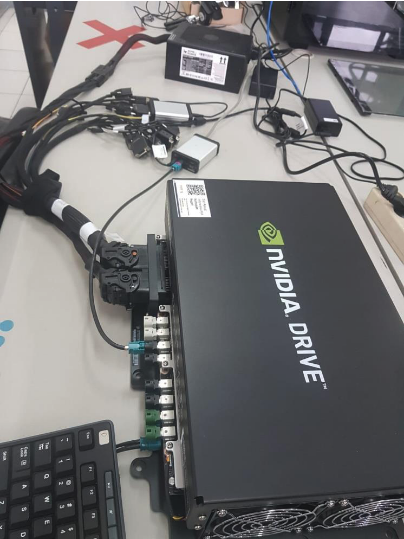
\includegraphics[height=0.5\textheight]{resources/chapter-2/pegasus.png}
        \caption{NVIDIA Pegasus \parencite{trilaksono_laporanRispro}}
    \end{center}
\end{figure}

Mengutip dari \parencite{oh_2017}, NVIDIA Pegasus adalah komputer yang
mendukung pengemudian \textit{autonomous} secara penuh. Artinya, NVIDIA Pegasus
dapat digunakan untuk membuat sebuah kendaraan bermotor menjadi
\textit{autonomous vehcile} jika sensor dan algoritma yang digunakan tepat.

NVIDIA Pegasus menggunakan 2 GPU dengan arsitektur post-Volta dan 2 SoC NVIDIA
Xavier. Kombinasi CPU dan GPU ini dapat menghasilkan 320 TOPS (\textit{trillion
    operations/second}) untuk komputasi intelegensi buatan. Untuk koneksi I/O,
NVIDIA Pegasus mendukung sampai dengan 16 kamera (6 di antaranya adalah lidar).

% TODO: Jelasin/masukin hubungannya dengan CARLA dan jelasin juga kalo NVIDIA
% Pegasus ini komputer biasa yang bisa menggunakan berbagai OS (buat transisi ke
% rosbridge)

\section{Metode Komunikasi antara Simulator CARLA dan NVI\-DI\-A Pegasus}

Pada keadaan yang ada, komunikasi antara simulator CARLA dengan NVIDIA Pegasus
menggunakan perantara \textit{web service} yang berbasis HTTP. Penggunaan HTTP
pada \textit{web service} menjadi \textit{bottleneck}/penghambat kinerja
terbesar sistem simulasi. Ketika dilakukan secara SILS (\textit{software in the
    loop simulation} tanpa NVIDIA Pegasus) didapatkan kinerja 4000 transaksi per
detik, sedangkan ketika NVIDIA Pegasus ditambahkan ke sistem (menjadi HILS,
\textit{hardware in the loop simulation}) didapatkan 100--110 transaksi per
detik \parencite{trilaksono_laporanRispro}. Oleh karena itu, dibutuhkan protokol
atau metode komunikasi lain yang dapat meningkatkan kinerja jalur komunikasi.
Selain itu, jalur komunikasi yang digunakan harus dapat mengirimkan pesan berupa
teks \textit{string}, larik angka, atau data \textit{binary} (misalnya gambar).

\begin{figure}
    \begin{center}
        \includegraphics[width=1.0\textwidth]{resources/chapter-2/komunikasi
            data pada simulasi.png}
        \caption{arsitektur komunikasi data pada HILS
            \parencite{trilaksono_laporanRispro}}
    \end{center}
\end{figure}

Beberapa alternatif metode/protokol jalur komunikasi dapat digunakan untuk
meng\-hu\-bung\-kan sistem ini akan dibahas pada subbab ini. Protokol atau
metode tersebut adalah rosbridge, RPC, dan \textit{messaging system}.

\subsection{Rosbridge}

Rosbridge adalah protokol komunikasi yang menambahkan antarmuka pada komputer
dengan sistem operasi ROS. Antarmuka yang ditambahkan membuat komputer dapat
\textit{publish} dan \textit{subscribe} ke topik ROS dalam format JSON. Selain
itu, antarmuka tersebut memungkinkan memanggil \textit{service} ROS di antara
hal-hal lainnya.

Spesifikasi lengkap untuk rosbridge tertuang di proyek \parencite{ros_bridge}.
Pada subbab ini, spesifikasi rosbridge akan dijelaskan secara singkat.

Secara arsitektur, protokol rosbridge menggunakan protokol WebSocket untuk
la\-pi\-san transpornya. Protokol WebSocket sendiri berjalan di atas protokol TCP
yang artinya protokol rosbridge menjamin data akan sampai dengan urutan yang
benar.

Protokol rosbridge menggunakan format JSON untuk pesannya. Pesan yang valid
harus mengandung \textit{field} \texttt{"op"}. \textit{Field} tersebut digunakan
untuk menentukan jenis pesan. Pesan juga dapat mengandung \textit{field}
\texttt{"id"} yang digunakan sebagai penanda transaksi atau keterhubungan antara
beberapa pesan. Selain kedua \textit{field} tersebut, pesan rosbridge juga dapat
mengandung \textit{field} lainnya tergantung jenis \texttt{"op"}.

\begin{lstlisting}[language=JSON, caption=contoh pesan valid pada lapisan
transpor rosbridge]
{
    "op": "fragment"
}
\end{lstlisting}

Jenis pesan yang dapat dikirim dapat dibagi menjadi 3 kategori.
Kategori-kategori tersebut akan diuraikan sebagai berikut.
\begin{enumerate}
    \item Pesan kompresi atau transformasi dengan kode \texttt{op}:
          \begin{itemize}
              \item \texttt{fragment} untuk pesan yang terpecah-pecah, atau
              \item \texttt{png} untuk pesan yang berupa berkas PNG.
          \end{itemize}
    \item Pesan status rosbridge:
          \begin{itemize}
              \item \texttt{set\_status\_level} untuk mengatur tingkat pelaporan
                    rosbridge, atau
              \item \texttt{status} untuk pesan status.
          \end{itemize}
    \item Pesan operasi:
          \begin{itemize}
              \item \texttt{advertise} untuk menandakan pengirim sedang
                    mempublikasikan suatu topik,
              \item \texttt{unadvertise} untuk menandakan pengirim berhenti
                    mempublikasikan suatu topik,
              \item \texttt{publish} untuk pesan ROS yang dipublikasikan ke
                    suatu topik,
              \item \texttt{subscribe} untuk meminta ``berlangganan'' ke suatu
                    topik,
              \item \texttt{unsubscribe} untuk meminta berhenti ``berlangganan'',
              \item \texttt{call\_service} untuk memanggil suatu layanan,
              \item \texttt{advertise\_service} untuk menandakan pengirim
                    sedang mem\-pu\-bli\-ka\-si\-kan suatu layanan, \item
                    \texttt{unadvertise\_service} untuk menandakan pengirim
                    berhenti mempublikasikan suatu layanan,
              \item \texttt{service\_request} untuk \textit{request}/permintaan
                    ke suatu layanan, atau \item \texttt{service\_response} untuk
                    hasil/balasan permintaan ke suatu layanan.
          \end{itemize}
\end{enumerate}

Pesan yang dikirim melalui protokol rosbridge dapat di-\textit{encode} dengan 3
format. Format pertama adalah \textit{raw} JSON. Dalam format ini, pesan yang
dikirim akan berupa \textit{string} biasa. Selain itu, pesan yang dikirim juga
dapat dikompresi dengan format CBOR (\textit{concise binary object
    representation}) atau CBOR-\textit{raw}. Pesan dalam format CBOR akan
berbentuk pesan \textit{binary}. Sehingga pesan harus didekompresi oleh
penerima untuk mendapatkan pesan aslinya.

Perbedaan antara CBOR dengan CBOR-\textit{raw} adalah format pesannya. Pada
CBOR-\textit{raw}, pesan dikirim dalam format serialisasi ROS. Format
serialisasi ROS digunakan untuk mengirimkan data antar-ROS \textit{node} dan
pada berkas \texttt{bag}\footnote{Format berkas yang digunakan untuk menyimpan
    data pada mesin ROS.}. Keuntungan menggunakan CBOR-\textit{raw} adalah
peningkatan kinerja jika \textit{parsing} hanya sebagian pesan, aplikasi dapat
membaca berkas \texttt{bag}, atau \textit{parsing} pesan ingin dilakukan
seterlambat mungkin atau secara paralel.

\subsection{RPC}

RPC, atau \textit{remote procedure call}, secara teknis bukanlah protokol,
melainkan sebuah mekanisme untuk menyusun sistem terdistribusi yang
berkomunikasi dengan pola \textit{request/reply}
\parencite{larry_computerNetwork}. RPC memberikan abstraksi kepada pengembang
berupa pemanggilan fungsi secara lokal maupun \textit{remote}, di permukaannya,
memiliki perilaku yang sama. Pemanggilan fungsi \textit{remote} artinya
implementasi fungsi berada di komputer lain di dalam jaringan.

Ketika menggunakan RPC, pengembang tidak perlu tahu pemanggilan sebuah fung\-si
dilakukan secara lokal atau \textit{remote}; pengembang hanya tahu pemanggilan
fungsi tersebut akan menghasilkan suatu nilai baru dan dapat (tidak
selalu\footnote{Beberapa implementasi RPC mendukung pemanggilan
    \textit{asynchronous} yang tidak harus memberikan sebuah \textit{return}
    (misalnya Apache Thrift dengan kata kunci \texttt{async}/\texttt{oneway}
    \parencite{agarwal_thrift}).})
membuat program \textit{blocking} (menunggu) sampai nilai baru tersebut
didapatkan.

Abstraksi RPC ``diberikan'' oleh 2 komponen utama pada RPC. Komponen pertama
adalah protokol yang mengurusi pengiriman pesan antara \textit{server/producer}
dan \textit{client/consumer}. Kedua, bahasa pemrograman dan \textit{compiler}
yang dapat membungkus pemanggilan fungsi \textit{remote} menjadi pesan
\textit{request} dan mentranslasikan pesan \textit{request} menjadi pemanggilan
ke fungsi lokal (begitu juga untuk \textit{return} dari pemanggilan fungsi
\textit{remote}).

Secara arsitektur, RPC bisa dibangun di atas protokol TCP sehingga pembuat
implementasi RPC tidak perlu memikirkan keandalan (\textit{reliability})
pengiriman pesan pada implementasinya. Akan tetapi, RPC juga bisa dibangun di
atas protokol UDP atau IP lalu ditambahkan/dibuat lapisan keandalannya sendiri.

Implementasi RPC yang akan dibahas pada subbab ini adalah Apache Thrift.
Apa\-che Thrift juga merupakan implementasi RPC yang akan digunakan untuk
membangun jalur komunikasi antara server NVIDIA Pegasus dengan server simulator
CARLA. Apache Thrift dipilih karena kemampuannya mengirimkan pesan dalam format
\textit{binary}. Selain itu, karena kinerja Apache Thrift lebih baik
dibandingkan dengan HTTP dan implementasi RPC oleh Google, gRPC
\parencite{abernethy_buildingHighPerformanceMSThrift}.

\subsubsection{Apache Thrift}

Apache Thrift adalah sebuah implementasi RPC dalam bentuk \textit{framework}
yang diciptakan oleh Facebook, Inc. (sekarang Meta Platforms, Inc.) lalu
disumbangkan ke Apache Software Foundation. Tujuan utama dari pembuatan Apache
Thrift adalah sebuah jembatan antar-bahasa pemrograman yang memiliki kinerja
tinggi \parencite{agarwal_thrift} sehingga Apache Thrift dapat digunakan lintas
bahasa pemrograman.

Apache Thrift memiliki beberapa abstraksi yang memudahkan pengembang untuk
menggunakan RPC. Abstraksi-abstraksi tersebut adalah sistem tipe, protokol,
transpor, pemberian versi, dan prosesor.

Sistem tipe pada Apache Thrift bertindak sebagai \textit{common language}
antar-bahasa pemrograman. Dengan adanya sistem tipe ini, sebuah definisi untuk
Apache Thrift dapat digunakan untuk banyak bahasa tanpa mengharuskan pemrogram
menulis tipe data buatan atau kode serialisasi sendiri. Tipe-tipe yang ada pada
sistem tipe Apache Thrift adalah \parencite{agarwal_thrift}
\begin{itemize}
    \item tipe dasar: \texttt{bool}, \texttt{byte}, \texttt{i16},
          \texttt{i32}, \texttt{i64}, \texttt{double}, dan \texttt{string},
    \item tipe struktur data (``\textit{struct}''): tipe komposit yang setara
          dengan kelas data pada pemrograman berorientasi objek atau \texttt{struct}
          pada C,
    \item \textit{container}: kumpulan data dan terdiri atas
          \begin{itemize}
              \item \texttt{list<type>}: daftar terurut dari beberapa elemen
                    dengan tipe \texttt{type},
              \item \texttt{set<type>}: himpunan elemen dengan tipe
                    \texttt{type} yang tidak terurut, dan
              \item \texttt{map<type1, type2>}: \textit{map} dengan \textit{key}
                    unik bertipe \texttt{type1} yang di\-pe\-ta\-kan tepat ke 1
                    \textit{value} bertipe \texttt{type2},
          \end{itemize}
    \item \textit{exception}: galat dan pendefinisiannya sama dengan
          \textit{struct}, dan
    \item layanan (``\textit{service}''): akan menciptakan \textit{interface}
          (atau padanannya) di bahasa target.
\end{itemize}

Data-data yang ingin digunakan pada sistem dan sesuai dengan sistem tipe Thrift
dapat dituliskan pada Thrift IDL (\textit{interface definition language}).
Thrift IDL memungkinkan pendefinisian struktur-struktur data tanpa harus
menuliskan informasi cara mentransportasikan data dengan aman. Struktur data
yang dapat didefinisikan pada Thrift IDL adalah \textit{struct}, \textit{enum},
konstanta (``\textit{const}''), alias tipe (\texttt{typedef} di C), \textit{union}
(\texttt{union} di C), dan \textit{exception}. IDL akan digunakan pembangkit
kode Thrift untuk membangkitkan kode pada bahasa target sehingga dapat
menggunakan layanan dan struktur data pada IDL.

Abstraksi transpor pada Apache Thrift membangkitkan kode yang dapat
di\-gu\-na\-kan untuk transpor data. Dengan adanya abstraksi ini, antarmuka
aliran data dapat dengan mudah diubah-ubah. Kode yang dibangkitkan Thrift juga
tidak peduli dengan sumber data sehingga dengan adanya abstraksi ini pengguna
Thrift dapat memilih media transpor data dengan bebas dan mudah.
\textit{Interface} untuk abstraksi transpor adalah \texttt{TTransport}.

Abstraksi protokol memisahkan struktur data dari representasi yang digunakan
untuk transpor. Dengan adanya abstraksi protokol, pengguna Thrift tidak perlu
me\-mi\-kir\-kan cara \textit{encoding} dan \textit{decoding} data yang ingin dikirim
melalui abstraksi transpor. \textit{Interface} untuk abstraksi protokol adalah
\texttt{TProtocol}.

Abstraksi \textit{versioning} bertujuan memudahkan pembaharuan layanan dan
struktur data. Abstraksi ini dicapai dengan penambahan sebuah nomor
\textit{identifier} sebelum \textit{field} pada \textit{struct} dan
\textit{exception} serta pada argumen untuk metode-metode layanan.

Abstraksi prosesor adalah abstraksi yang untuk memproses data dan melakukan RPC.
Abstraksi prosesor menggunakan \textit{interface} \texttt{TProcessor} dan
memiliki sebuah metode \texttt{process} untuk menangani pemanggilan RPC.

Thrift juga menyediakan sebuah \textit{interface} \texttt{TServer}.
\texttt{TServer} bertanggung jawab atas pengurusan koneksi, \textit{threading},
dll. sedangkan \texttt{TProcessor} bertanggung jawab atas penanganan pemanggilan
RPC. Salah satu pekerjaan \texttt{TServer} adalah memanggil metode
\texttt{process} pada \texttt{TProcessor}.

\textit{Interface} \texttt{TServer} dan \texttt{TProcessor} akan dibangkitkan
pada server/produsen. Se\-dang\-kan pada klien/konsumen akan dibangkitkan
implementasi untuk \textit{interface}/la\-ya\-nan pada IDL, disebut
\textit{client}. Implementasi pada klien memanfaatkan 2 buah \texttt{TProtocol}
untuk melakukan proses I/O.

\begin{figure}
    \begin{center}
        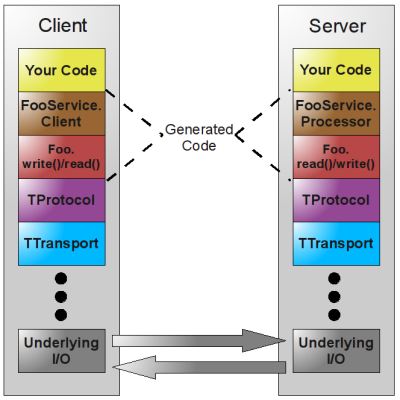
\includegraphics[width=0.25\textheight]{resources/chapter-2/thrift-arch.png}
        \caption{arsitektur Apache Thrift \parencite{prunicki_thrift}}
    \end{center}
\end{figure}

Secara bawaan, Apache Thrift mendukung beberapa transpor, protokol, dan server
\parencite{prunicki_thrift}. Dukungan-dukungan tersebut adalah
\begin{itemize}
    \item transpor (implementasi \texttt{TTransport}):
          \begin{itemize}
              \item \texttt{TSim\-ple\-FileTrans\-port}: menggunakan berkas,
              \item \texttt{TMe\-mo\-ry\-Trans\-port}: menggunakan memori,
              \item \texttt{T\-Sock\-et}: \textit{socket blocking},
              \item \texttt{TFramed\-Trans\-port}: pada server
                    \textit{nonblocking}, dan
              \item \texttt{T\-Z\-lib\-Trans\-port}: Melakukan kompresi dengan
                    zlib dan harus digunakan dengan trans\-por lain,
          \end{itemize}
    \item protokol (implementasi \texttt{TProtocol}):
          \begin{itemize}
              \item \texttt{TBinaryProtocol}: pesan dikirim dalam format
                    \textit{binary},
              \item \texttt{TCompactProtocol}: \texttt{TBinaryProtocol} yang
                    lebih \textit{compact},
              \item \texttt{TDenseProtocol}: \texttt{TCompactProtocol} yang
                    di\-hi\-lang\-kan \textit{me\-ta\-da\-ta}-nya, lalu ditambahkan
                    lagi oleh penerima,
              \item \texttt{TJsonProtocol}: pesan dikirim dalam format JSON,
              \item \texttt{TSimpleJsonProtocol}: \texttt{TJsonProtocol} tanpa
                    \textit{metadata}, cocok untuk bahasa \textit{scripting}, dan
              \item \texttt{TDebugProtocol}: format paling mudah dibaca manusia,
          \end{itemize}
    \item server (implementasi \texttt{TServer}):
          \begin{itemize}
              \item \texttt{TSimpleServer}: server \textit{single-threaded},
              \item \texttt{TThreadPoolServer}: server \textit{multi-threaded}
                    dengan \textit{blocking} I/O, dan
              \item \texttt{TNonBlockingServer}: server \textit{multi-threaded}
                    dengan \textit{non-blocking} I/O dan harus menggunakan
                    \texttt{TFramedTransport}.
          \end{itemize}
\end{itemize}

\subsection{\textit{Messaging System}}

\subsubsection{ZeroMQ}

\section{Penelitian Terkait}
\blindtext
\chapter{Analisis dan Rancangan Sistem HILS}\label{chapter-3}

Pada Bab \ref{chapter-3} akan dibahas analisis permasalahan pada sistem simulasi yang sudah
ada. Setelah itu, akan dilakukan analisis dan perancangan terhadap solusi yang
akan dibuat pada buku ini.

\section{Deskripsi Umum Proyek \textit{Capstone}}

Tugas akhir yang dikerjakan oleh tim \textit{capstone} bertujuan untuk memenuhi
kebutuhan tim simulasi pada proyek pengembangan trem otonom. Tim simulasi
dibentuk agar pengujian algoritma kendali dan pengumpulan data tidak harus
dilakukan dengan trem yang nyata. Alasannya adalah untuk keamanan, menghemat
biaya, dan menghemat waktu. Pengujian nyata dengan algoritma yang belum siap
dapat menyebabkan orang atau kendaraan lain ditabrak oleh trem. Selain itu,
dengan simulasi para pengembang tidak perlu terjun ke lapangan di Kota Madiun
dan tidak perlu menyewa trem serta rel untuk melakukan pengujian.

Proyek pengembangan trem otonom sendiri dan tim simulasi sudah memasuki tahun
kedua. Akan tetapi, sistem HILS yang ada memiliki banyak masalah, di antaranya
adalah belum adanya skenario simulasi dan kinerja sistem yang buruk. Oleh
karenanya, tim \textit{capstone} perlu memperbarui sistem HILS agar pengujian
HILS dapat dilakukan. Selain itu, tim \textit{capstone} ini juga harus membuat
lingkungan simulasi yang semirip mungkin dengan keadaan di Indonesia serta
membuat beberapa skenario simulasi agar pengujian dapat dilakukan secara
otomatis.

Tugas akhir ini sendiri bertujuan untuk memperbaiki agar sistem HILS dapat
menggunakan sensor virtual dan memiliki dengan kinerja yang baik.  Sistem HILS
sendiri sudah pernah diimplementasi pada tahun pertama proyek, akan tetapi
implementasinya memiliki beberapa keluhan yang akan dibahas pada Subbab
\ref{chapter-3-problems}. Dari keluhan-keluhan tersebut, akan dilakukan analisis
serta rancangan solusi untuk memperbaiki sistem HILS yang ada.

\section{Analisis Masalah Sistem HILS Saat ini}\label{chapter-3-problems}

Sistem simulasi yang ada sudah dapat menghubungkan komputer SILS dengan server
komputer RKB/AGX sehingga sistem HILS sudah dapat digunakan. Akan tetapi masih
ada keluhan terkait kinerja sistem HILS, yaitu proses simulasi yang sangat
lambat, menyebabkan simulasi kurang realistis. Jumlah transaksi data per
detik turun dari 4000 transaksi data per detik pada SILS, turun menjadi 100-110
transaksi data per detik ketika menggunakan HILS dan layanan web. Dari ketua tim
simulasi, target kecepatan simulasi yang harus dicapai untuk dianggap cukup
cepat adalah CARLA dapat berjalan stabil dengan minimum 2 FPS (\textit{frames
	per second}).

Padahal kedua komputer pada sistem HILS sudah terhubung pada jaringan lokal
(LAN) yang artinya latensi dan gangguan jaringan akan minimum, jika ada.
Oleh karena itu, kemungkinan \textit{bottleneck} terdapat pada implementasi
mekanisme komunikasi. Implementasi mekanisme komunikasi menggunakan sebuah
layanan web yang arsitekturnya dapat dilihat pada diagram di Gambar
\ref{chapter-2-old-hils}. Proses pada sistem HILS yang sudah ada dapat dilihat
pada diagram sekuens di Gambar \ref{chapter-3-sequence-diagram-old-hils}. Pada
proses pengiriman data, terdapat delapan operasi I/O yang berjalan secara
sinkronis, yaitu
\begin{enumerate}
	\item penulisan CARLA \textit{measurement} ke \textit{file} di SILS,
	\item pembacaan CARLA \textit{measurement} dari \textit{file} di SILS,
	\item pengiriman CARLA \textit{measurement} menggunakan HTTP dari SILS ke
	      layanan web,
	\item penulisan CARLA \textit{measurement} ke basis data pada layanan web,
	\item permintaan HTTP dari AGX/RKB ke layanan web untuk membaca data,
	\item pembacaan CARLA \textit{measurement} dari basis data pada layanan web,
	\item penulisan CARLA \textit{measurement} ke \textit{file} pada AGX/RKB,
	      dan
	\item pembacaan CARLA \textit{measurement} dari \textit{file} pada AGX/RKB.
\end{enumerate}

\begin{figure}[h!]
	\centering
	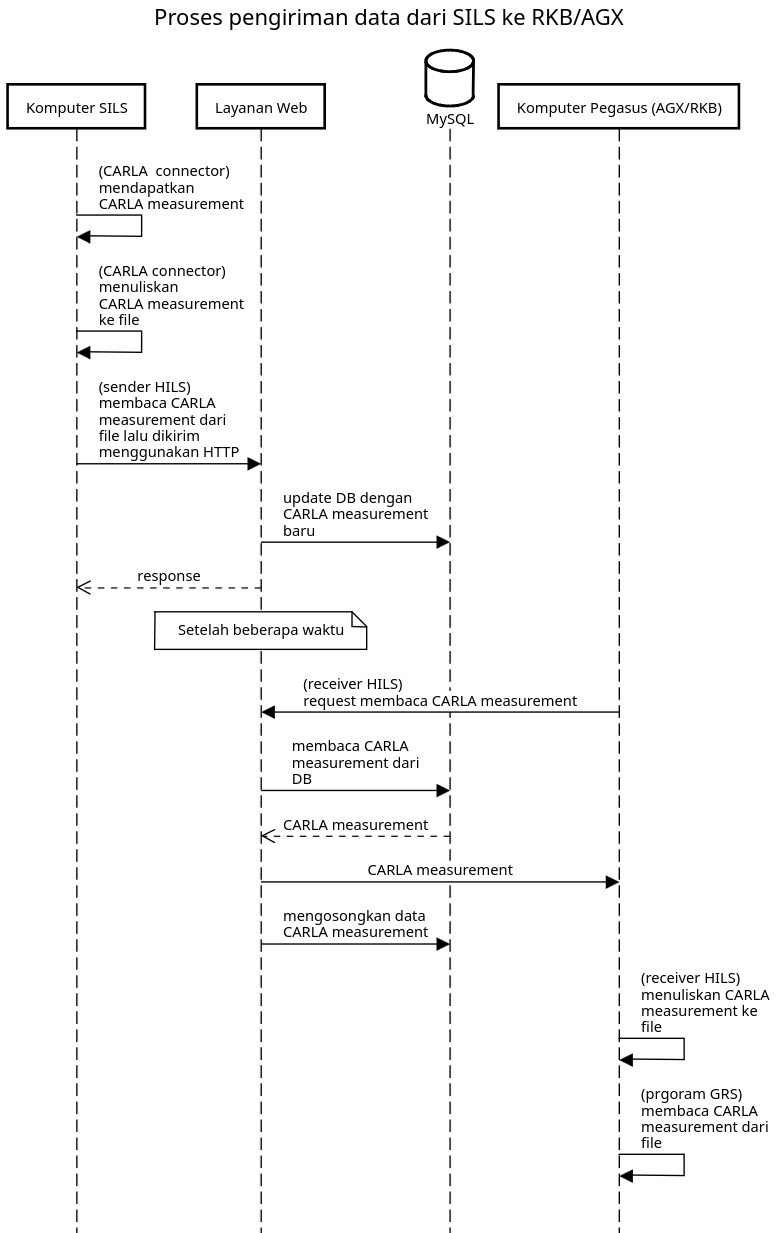
\includegraphics[width=1.0\textwidth]{resources/chapter-3/sequence-diagram-old-hils-process.png}
	\caption{Proses pengiriman data CARLA \textit{measurement} kondisi saat ini}
	\label{chapter-3-sequence-diagram-old-hils}
\end{figure}

Dari diagram sekuens dapat diperkiran \textit{bottleneck} disebabkan
banyaknya operasi I/O sinkronis yang berdampak pada \textit{overhead} operasi
I/O. \textit{Overhead} operasi I/O akan menjadi lebih buruk lagi apabila data
yang dikirimkan berukuran besar, misalnya data sensor kamera. Selain itu, sistem
yang ada juga lebih rumit dari seharusnya. Terdapat perantara berupa layanan web
dan basis data padahal data bisa saja dikirimkan langsung dari komputer SILS ke
komputer AGX/RKB.

Selain masalah kinerja, terdapat keluhan juga karena sistem HILS yang ada belum
menggunakan data sensor. Sistem HILS yang ada masih memanfaatkan CARLA
\textit{measurement}. Data dari CARLA \textit{measurement} mencakup posisi x,
posisi y, kecepatan, dan jarak relatif. Data-data ini dibutuhkan untuk
mendapatkan oleh algoritma kendali, akan tetapi seharusnya didapatkan dari
sensor. Pada sistem HILS saat ini, data \textit{measurement} tersebut didapatkan
dengan memanggil fungsi dari API Python CARLA.

\section{Analisis Solusi}

Dari analisis masalah, didapatkan dua keluhan pada sistem HILS yang ada, yaitu
masalah kinerja dan belum ada dukungan terhadap data sensor. Dari
keluhan-keluhan tersebut, dibutuhkan sebuah solusi yang dapat meningkatkan
kinerja HILS dan dapat menggunakan data sensor. Sensor-sensor yang harus
didukung pada solusi adalah sensor kamera, lidar, dan GNSS. Ketiga sensor harus
dapat digunakan secara bersamaan.

Dari kebutuhan-kebutuhan tersebut, ada dua buah alternatif solusi: melakukan
peningkatan (\textit{upgrade}) sistem HILS yang sudah ada atau menulis ulang
sistem HILS. Dari kedua alternatif, dipilih alternatif penulisan ulang program
HILS. Alasannya adalah karena pada solusi pertama memiliki kompleksitas yang
lebih tinggi karena ada lebih banyak komponen pada sistem. Selain itu, layanan
web pada solusi pertama tidak terintegrasi langsung pada program utama, baik di
komputer SILS maupun komputer AGX/RKB. Layanan web membutuhkan program bantuan
yang berkomunikasi dengan program utama menggunakan \textit{file}. Hal ini ingin
dihindari karena adanya \textit{overhead} I/O. Selain itu, meskipun layanan web
memiliki \textit{coupling} yang rendah dengan kedua program utama, kohesinya
juga rendah. Karena kedua alasan itulah dinilai alternatif kedua akan lebih
mudah untuk dilaksanakan.

Selanjutnya adalah pemilihan mekanisme komunikasi. Berdasarkan studi literatur,
terdapat dua alternatif untuk mekanisme komunikasi, yaitu ROS dan ZeroMQ. ROS
sendiri adalah salah satu kerangka kerja dan mekanisme komunikasi yang sering
digunakan untuk kebutuhan simulasi robot. Akan tetapi, karena kendala teknis ROS
tidak dapat dipilih. Oleh karena itu, dari pilihan antara ROS dan ZeroMQ,
dipilih ZeroMQ.

Kendala teknis yang menyebabkan ROS tidak dapat digunakan adalah ketidakcocokan
antara versi ROS di komputer SILS dengan komputer AGX/RKB. Komputer SILS
menggunakan sistem operasi Ubuntu 20.04 yang menggunakan ROS 2, sedangkan
komputer AGX/RKB menggunakan sistem operasi Ubuntu 18.04 yang menggunakan ROS 1.
ROS 2 dan ROS 1 memiliki arsitektur komunikasi yang berbeda, hal ini menyebabkan
ketidakcocokan antara ROS 2 dengan ROS 1. Meskipun ada program untuk
menjembatani ROS 2 dan ROS 1, hal tersebut dihindari karena adanya kemungkinan
penambahan latensi.

\section{Rancangan Solusi}

Karena program utama di sisi komputer SILS dan AGX/RKB sudah ada atau sedang
dikerjakan, dipilih solusi dalam bentuk pustaka agar pemuatan fungsionalitas
HILS bisa dilakukan secara modular dan independen dari kedua program utama.
Hal ini menciptakan \textit{coupling} yang rendah antara pustaka dengan kedua
program utama. Selain itu, keuntungan pustaka adalah program GRS jadi dapat
memilih untuk memuat pustaka yang akan dibuat atau tidak pada proses kompilasi
sehingga dapat sedikit menghemat \textit{resource} terutama memori. Pustaka yang
dibuat akan disebut ``hils-connector''.

Pustaka yang akan dibuat ada dua, yaitu pustaka C++11 untuk program GRS di
komputer AGX/RKB dan pustaka Python 3 untuk \textit{agent} program
\textit{scenario runner}. Pustaka Python akan disebut ``\textit{producer}''
karena memproduksi data sensor. Pustaka C++ akan disebut ``\textit{consumer}''
karena mengonsumsi data sensor. Selain data sensor, juga akan ada data berupa
kontrol/perintah dengan format sebuah \texttt{int} yang dikirim dari
\textit{consumer} ke \textit{producer} setelah data sensor berhasil diproses.

Lalu untuk fitur pustaka itu sendiri, pustaka akan langsung berkomunikasi satu
sama lain tanpa menggunakan perantara. Hal ini membuat solusi lebih sederhana
dan mengurangi \textit{overhead} untuk berkomunikasi dengan perantara. Pustaka
juga akan menyediakan API untuk mengirimkan data dan menerima data. Untuk
mendukung berbagai jenis sensor, pustaka juga akan memiliki fitur
\textit{parsing}, serialisasi, dan deserialisasi untuk sensor GNSS, kamera, dan
lidar.

API yang disediakan oleh pustaka ``producer'' akan langsung mengkonsumsi data
sensor dari CARLA sehingga pengguna pustaka tidak perlu melakukan modifikasi
apapun pada data sensor CARLA. Begitu juga pada pustaka ``consumer''. Balikan
API akan disesuikan sehingga pengguna pustaka dapat langsung menggunakan data
sensor dan langsung ``memasukkannya'' ke sensor virtual NVIDIA DriveWorks.

Lalu, untuk mengurangi berbagai \textit{overhead} tambahan yang dapat muncul
karena operasi pada jaringan, dipilih mekanisme komunikasi menggunakan ZeroMQ.
ZeroMQ adalah \textit{message queue} sehingga cocok digunakan untuk operasi
asinkron yang sesuai dengan pengiriman data sensor dari CARLA. Lalu, ZeroMQ juga
sangat dekat dengan TCP, tapi tanpa kompleksitas \textit{raw} TCP. Hal tersebut
dikarenakan salah satu tujuan utama ZeroMQ adalah mengurangi latensi hinga
sesedikit mungkin dan memaksimalkan \textit{throughput}. ZeroMQ juga tidak
memiliki \textit{broker}, hal ini sesuai dengan keinginan menghilangi perantara
sehingga \textit{producer} dan \textit{consumer} dapat langsung berkomunikasi
satu sama lain.

Dari solusi pustaka yang ditawarkan, dapat dibentuk sebuah arsitektur sistem
HILS. Arsitektur ini dapat dilihat pada diagram \textit{deployment} di Gambar
\ref{chapter-3-new-architecture}. Lalu, gambaran kasar proses pada sistem
simulasi untuk satu \textit{step} simulasi dapat dilihat pada diagram
\textit{sequence} di Gambar \ref{chapter-3-new-sequence}. Perlu dicatat bahwa
HILS \textit{agent} adalah \textit{agent} yang digunakan pada program
ScenarioRunner.

\begin{figure}[!htbp]
	\centering
	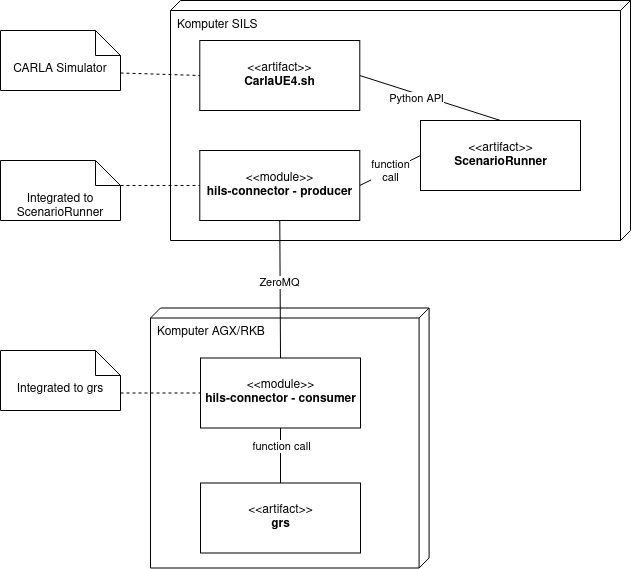
\includegraphics[width=1.0\textwidth]{resources/chapter-3/deployment-diagram-new-hils.png}
	\caption{Arsitektur Sistem HILS Baru}
	\label{chapter-3-new-architecture}
\end{figure}

\begin{figure}[!htbp]
	\centering
	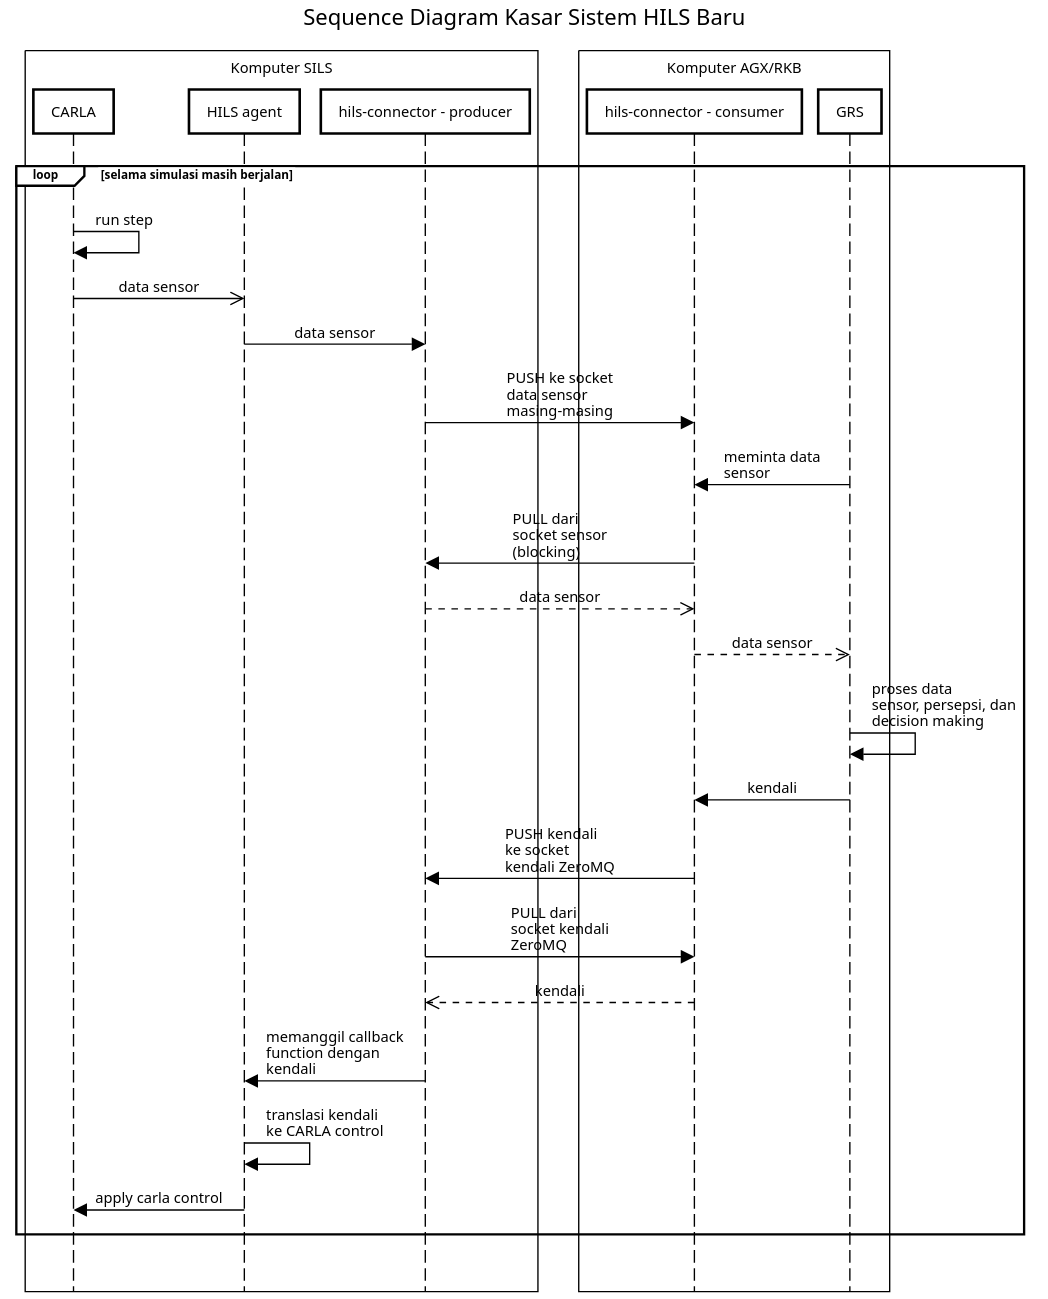
\includegraphics[width=1.0\textwidth]{resources/chapter-3/sequence-diagram-new-hils-kasar.png}
	\caption{Gambaran kasar proses satu \textit{step} simulasi}
	\label{chapter-3-new-sequence}
\end{figure}

\chapter{Implementasi dan Pengujian Pustaka Sistem HILS}\label{chapter-4}

\section{Implementasi Pustaka Sistem HILS}

Berdasarkan analisis dan rancangan solusi pada Bab \ref{chapter-3}, dapat
dimulai implementasi pustaka sistem HILS baru. Implementasi pustaka dimulai
dengan eksplorasi ROS2 dan ZeroMQ. Kemudian dilanjutkan dengan pembuatan program
\textit{proof of concept} (POC) menggunakan salah satu mekanisme komunikasi. POC
dibuat untuk menunjukan bahwa mekanisme komunikasi yang digunakan dapat
melakukan transfer data kamera sehingga CARLA berjalan dengan setidaknya 2 FPS.
Setelah POC diterima oleh ketua tim simulasi, dilanjutkan penulisan pustaka
\textit{consumer} dan terakihir implementasi pustaka \textit{producer}.

Dari proses eksplorasi dan implementasi POC, didapatkan metode komunikasi yang
cocok adalah ZeroMQ. ROS 2 sendiri gagal pada tahap POC dikarenakan sistem
operasi tidak kompatibel dengan ROS 2. Oleh karena itu, implementasi pustaka
akan menggunakan ZeroMQ. Sedangkan, ROS 2 tidak akan digunakan lagi pada tugas
akhir ini.

Pustaka yang pertama ditulis adalah pustaka \textit{consumer} (sisi
komputer AGX/RKB) karena program utama komputer SILS (pengguna
\textit{producer}) belum selesai pada saat proses penulisan pustaka. Akibatnya,
pengujian pustaka \textit{consumer} lebih mudah dilakukan pada saat itu.

Pustaka \textit{producer} dan \textit{consumer} akan memanfaatkan pemrograman
berorientasi objek untuk menstruktur kodenya. Pustaka yang dibuat juga dibuat
seabstrak mungkin dan tidak \textit{coupled} pada trem saja. Sehingga pustaka
yang ditulis dapat digunakan untuk simulasi \textit{hardware-in-the-loop} jenis
kendaraan otonom lainnya.

Diagram kelas dari pustaka \textit{consumer} dapat dilihat pada gambar
\ref{chapter-4-consumer-class-diagram}. Kelas yang melakukan komunikasi adalah
kelas abstrak \texttt{Endpoint}. Kelas tersebut dibuat abstrak dan diinstansiasi
menggunakan pola pemrograman \textit{factory}. \texttt{Endpoint} dibuat abstrak
agar apabila ingin ditambahkan metode komunikasi lain, hal tersebut dapat
dilakukan dengan mudah. Contoh kasus penggunaan penambahan metode komunikasi
lain adalah pengujian atau \textit{benchmarking} metode komunikasi. Selain itu,
terdapat kelas yang akan menyediakan layanan untuk program GRS, yaitu
\texttt{CarlaService}. Kelas ini mengabstraksi komunikasi dan deserialisasi
ataupun serialisasi data dari \texttt{Endpoint}.
\begin{figure}[!htbp]
	\centering
	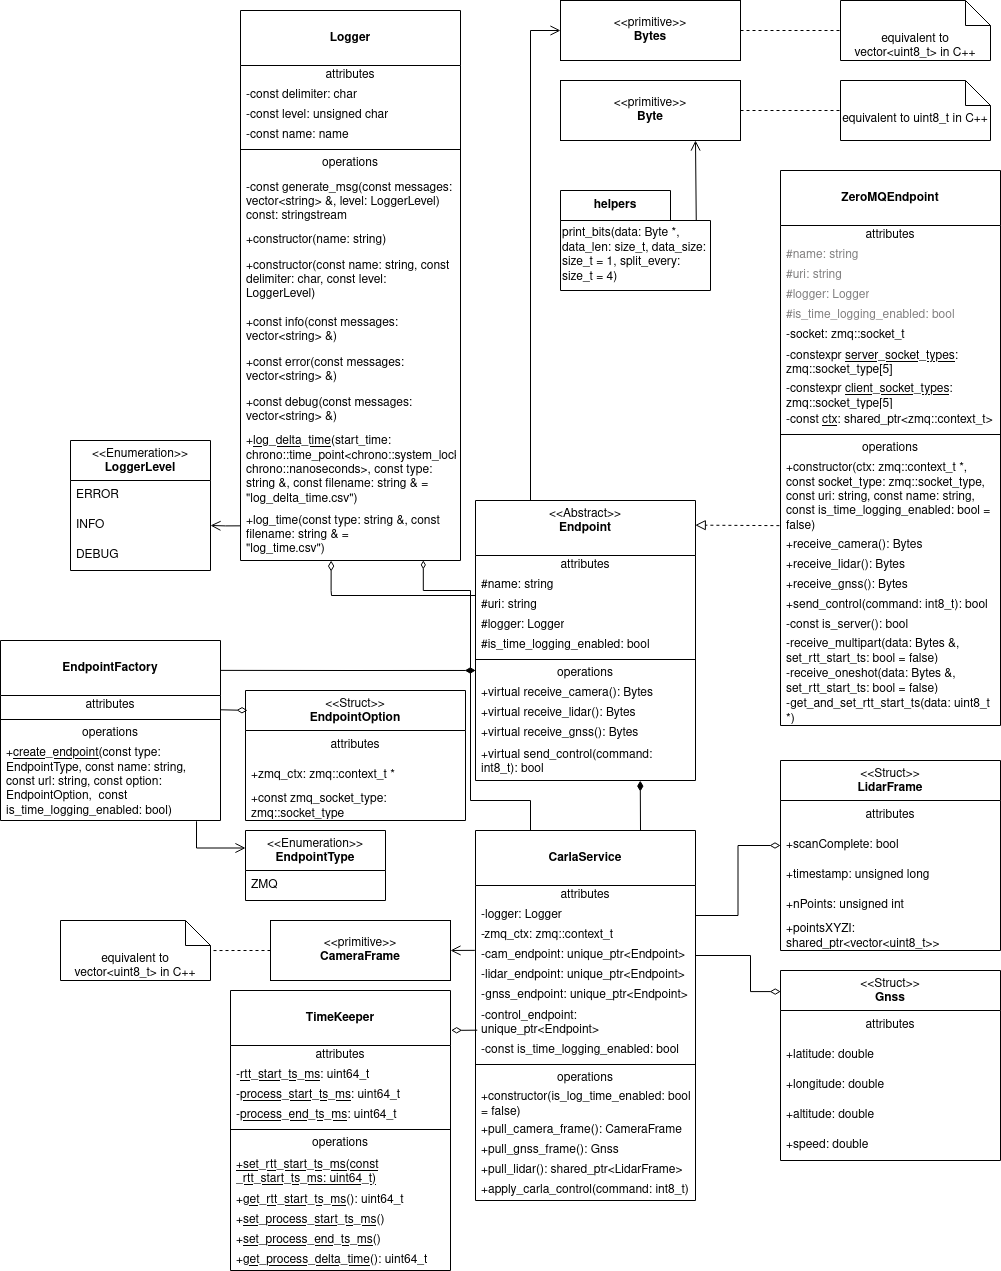
\includegraphics[width=1.0\textwidth]{resources/chapter-4/consumer-class_diagram.png}
	\caption{Diagram Kelas Pustaka \textit{Consumer}}
	\label{chapter-4-consumer-class-diagram}
\end{figure}

Setelah pustaka \textit{consumer} berhasil, implementasi dilanjutkan dengan
pembuatan pustaka \textit{producer}. Diagram kelas pustaka \textit{producer}
dapat dilihat pada gambar \ref{chapter-4-producer-class-diagram}. Pembuatan
pustaka \textit{producer} juga mengikuti filosofi penulisan pustaka
\textit{consumer}. Pustaka dibuat seabstrak mungkin sehingga tidak
\textit{coupled} dengan trem. Kelas \texttt{Endpoint} juga dibuat abstrak agar
dapat ditambahkan metode komunikasi yang lain. Perbedaan implementasi adalah
pada kelas yang berinteraksi dengan program utama. Pada pustaka
\textit{producer}, ada empat kelas yang berinteraksi dengan program utama, yaitu
\texttt{CameraHandler}, \texttt{LidarHandler}, \texttt{GnssHandler}, dan
\texttt{ControlHandler}. Keempat kelas memiliki peran masing-masing dan
terspesialisasi untuk menangani data dari sensor virtual CARLA tertentu.
\begin{figure}[!htbp]
	\centering
	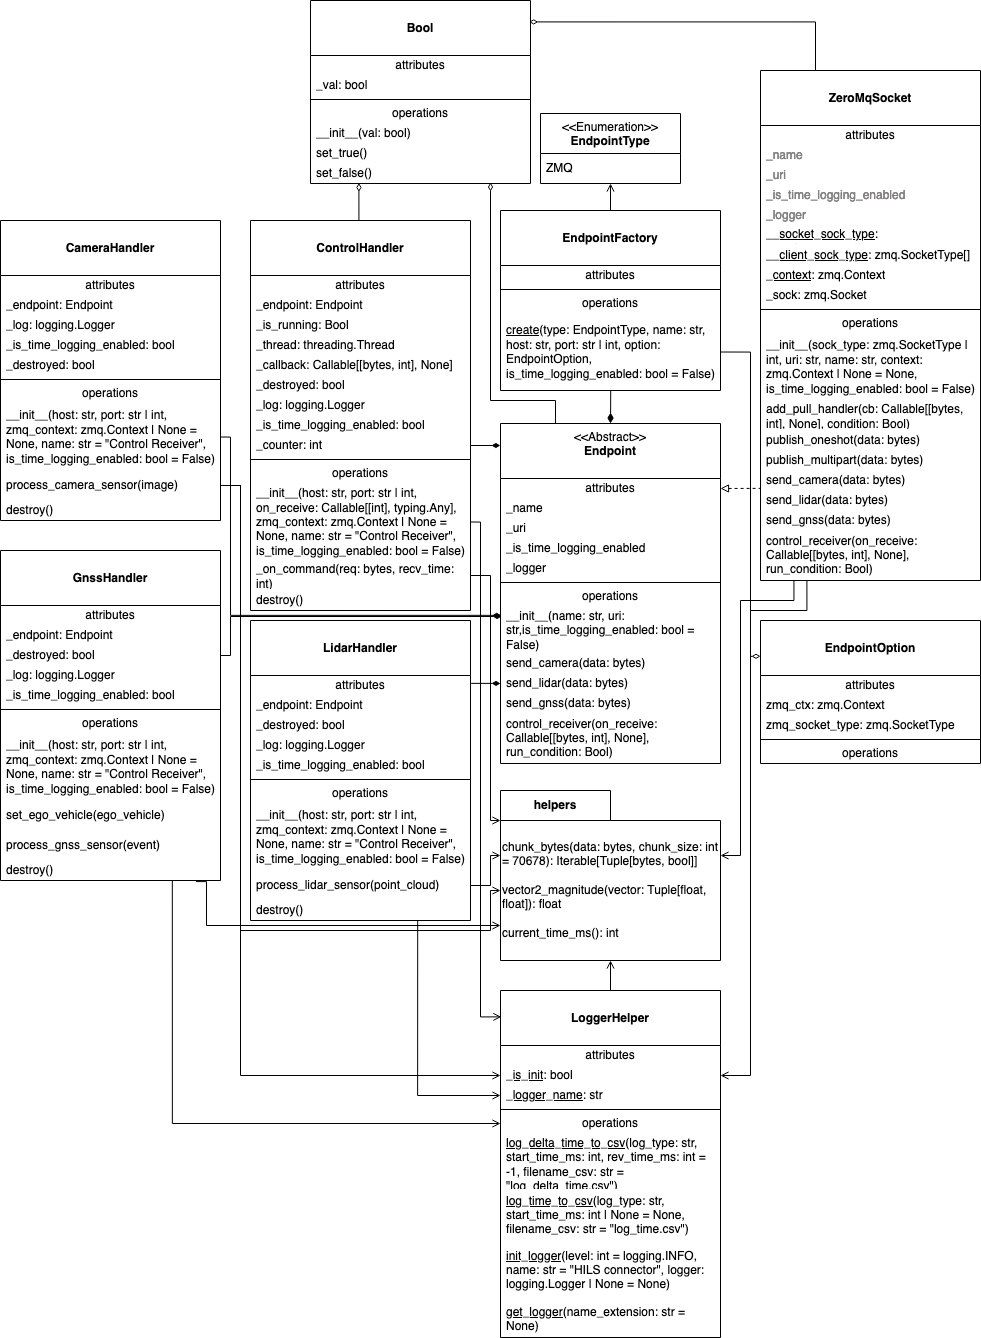
\includegraphics[width=1.0\textwidth]{resources/chapter-4/producer-class_diagram.png}
	\caption{Diagram Kelas Pustaka \textit{Producer}}
	\label{chapter-4-producer-class-diagram}
\end{figure}

Setelah kedua pustaka diimplementasi, dilakukan pengujian pustaka dengan program
kecil. Lalu, kedua pustaka diintegrasi dengan kedua program utama. Setelah itu,
dapat dianggap sistem implementasi HILS yang baru sudah diimplementasi dan
pengujian HILS dapat dilakukan. Akan tetapi untuk kebutuhan tugas akhir, sebelum
pengujian HILS dilakukan, akan dilaksanakan pengujian. Metode pengujian dan
aspek sistem yang diuji akan dibahas pada Subbab
\ref{chapter-4-testing-methodology}.

\section{Metode Pengujian Implementasi dan
  Kinerja}\label{chapter-4-testing-methodology}

Pengujian akan menguji dua aspek, yaitu
\begin{enumerate}
	\item pengujian implementasi: meninjau kemampuan pustaka dalam mengirim,
	      menerima, dan menggunakan data dari sensor virtual untuk
	      mengendalikan trem; dan
	\item pengujian kinerja: meninjau latensi yang dibutuhkan untuk mengirim
	      data dan meninjau kecepatan simulator saat simulasi.
\end{enumerate}
Subbab \ref{chapter-4-testing-methodology}, akan membahas metode dan rencana
pengujian kedua aspek tersebut. Selain itu, akan dibahas juga lingkungan
pengujian. Pengujian dilakukan dengan menjalankan beberapa skenario simulasi
lalu dibandingkan dengan kriteria kedua aspek. Sebuah aspek dinyatakan berhasil
apabila semua kriterianya berhasil dicapai.

\subsection{Lingkungan Pengujian}

Pengujian pustaka dan sistem HILS dilakukan pada laboratorium sistem kendali di
Lab Teknologi VIII ITB. Komputer yang akan digunakan pada lab tersebut ada tiga,
yaitu komputer AGX, komputer RKB, dan komputer SILS. Komputer AGX adalah NVIDIA
Drive PX Pegasus. Spesifikasi komputer AGX dapat dilihat pada Subbab
\ref{chapter-2-section-pegasus}. Sedangkan spesifikasi komputer SILS dan RKB
adalah sebagai berikut (Tabel \ref{chapter-4-tbl-environment-specs}).

\begin{table}[!htbp]
	\centering
	\begin{tabular}{|r|l|l|}
		\hline
		                  & CPU & i9-10920X 12C/24T 3.50GHz  \\
		\cline{2-3}
		\textbf{Komputer} & RAM & 128GB                      \\
		\cline{2-3}
		\textbf{SILS}     & GPU & 2x NVIDIA GeForce RTX 3090 \\
		\cline{2-3}
		                  & OS  & Ubuntu Linux 20.04         \\
		\hline
		                  & CPU & i7-8700 6C/12T 3.20GHz     \\
		\cline{2-3}
		\textbf{Komputer} & RAM & 16GB                       \\
		\cline{2-3}
		\textbf{RKB}      & GPU & NVIDIA GeForce RTX 2070    \\
		\cline{2-3}
		                  & OS  & Ubuntu Linux 18.04         \\
		\hline
	\end{tabular}
	\caption{Spesifikasi komputer SILS dan komputer RKB.}
	\label{chapter-4-tbl-environment-specs}
\end{table}

Untuk pengujian implementasi, akan dilakukan pada komputer AGX dan komputer
SILS. Komputer AGX akan menjalankan program GRS dan komputer SILS akan
menjalankan program ScenarioRunner. Sedangkan pada pengujian kinerja komputer
yang akan digunakan adalah komputer RKB. Komputer RKB akan menggantikan fungsi
komputer AGX.

Pada pengujian kinerja, kedua komputer (komputer RKB dan komputer SILS)
terhubung pada sebuah jaringan lokal (LAN). Topologi jaringan dapat dilihat di
Gambar \ref{chapter-4-fig-topology}. Komputer SILS dan komputer RKB terhubung
melalu sebuah \textit{switch} HPE JH019A. Komputer SILS terhubung ke
\textit{switch} menggunakan sebuah cabel Cat5. Sedangkan komputer RKB terhubung
ke \textit{switch} menggunakan sebuah cabel Cat6 bermerk Commscope 1071E.
Kecepatan \textit{link} pada kedua komputer adalah 1 Gbps.

\begin{figure}[!htbp]
	\centering
	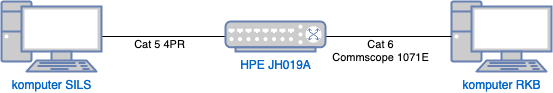
\includegraphics[width=1.0\textwidth]{resources/chapter-4/test-environment-network-topology.png}
	\caption{Topologi lingkungan pengujian}
	\label{chapter-4-fig-topology}
\end{figure}

\subsection{Pengujian Implementasi Pustaka}

Pengujian implementasi dilakukan dengan menjalankan program utama di komputer
SILS dan komputer AGX/RKB. Kemudian, akan dilakukan observasi untuk memeriksa
pustaka sudah memenuhi kriteria-kriteria pada Tabel
\ref{chapter-4-tbl-impl-criteria} atau belum.

\begin{table}[!htbp]
	\begin{center}
		\begin{tabular}{|l|l|}
			\hline
			\textbf{Kode} & \textbf{Deskripsi}                                     \\
			\hline
			IMPL-01       & Kecepatan trem di program GRS sesuai dengan bacaan
			sensor                                                                 \\
			              & GNSS.                                                  \\
			\hline
			IMPL-02       & Tampilan kamera di program GRS sesuai dengan yang
			ada di                                                                 \\
			              & program ScenarioRunner.                                \\
			\hline
			IMPL-03       & Tampilan lidar di program GRS menampikan
			objek-objek                                                            \\
			              & yang ada di sekitar trem.                              \\
			\hline
			IMPL-04       & Trem maju ketika mendapatkan kendali maju dan berhenti \\
			              & ketika mendapatkan kendali berhenti.                   \\
			\hline
		\end{tabular}
	\end{center}

	\caption{Kriteria pengujian implementasi pustaka}
	\label{chapter-4-tbl-impl-criteria}
\end{table}

Kriteria ini selaras dengan tujuan tugas akhir yang kedua, yaitu
mengimplementasikan mekanisme komunikasi sistem simulasi yang dapat mengirimkan,
menerima, dan memanfaatkan data dari berbagai jenis sensor.

\subsection{Pengujian Kinerja Mekanisme Komunikasi Pustaka}

Dari segi kinerja, hal yang ingin dipastikan adalah CARLA dapat berjalan stabil
dengan kecepatan minimum 2 FPS (\textit{frames per second}). Hal tersebut
diobservasi dengan menjalankan kedua program utama. Selain dari kecepatan
simulator, aspek kinerja juga akan dinilai dari perbandingan dengan mekanisme
komunikasi sistem HILS yang ada. Latensi pengiriman data harus lebih rendah
dibandingkan latensi sistem HILS yang ada. Kedua kriteria tersebut dituangkan
pada Tabel
\ref{chapter-4-tbl-perf-criteria}.
\begin{table}[!htbp]
	\begin{center}
		\begin{tabular}{|l|l|}
			\hline
			\textbf{Kode} & \textbf{Deskripsi}                                       \\
			\hline
			              & CARLA dapat berjalan dengan stabil dengan kecepatan      \\
			PERF-01       & minimum 2 FPS ketika simulasi menggunakan sensor         \\
			              & kamera dan GNSS.                                         \\
			\hline
			PERF-02       & Latensi pengiriman data lebih rendah dibandingkan sistem \\
			              & HILS yang ada.                                           \\
			\hline
		\end{tabular}
	\end{center}
	\caption{Kriteria pengujian kinerja mekanisme komunikasi sistem HILS}
	\label{chapter-4-tbl-perf-criteria}
\end{table}

Pengujian kriteria PERF-02 akan menggunakan \textit{round-trip time} (RTT) yang
dibagi dua untuk perkiraan latensi sistem. Rumus perhitungan RTT dapat dilihat
pada persamaan \ref{chapter-4-eq-rtt}.
\begin{equation}
	\label{chapter-4-eq-rtt}
	\text{RTT} = T_{e} - T_{s} - t_p
\end{equation}

Dengan keterangan persamaan sebagai berikut.
\begin{table}[!h]
	\begin{tabular}{l l}
		RTT     & :     \textit{round-trip time} (dalam ms)             \\
		$T_{e}$ & : \textit{timestamp} didapatkan kendali (dalam ms)    \\
		$T_{s}$ & : \textit{timestamp} dikirimkan segmen pertama kamera
		(dalam ms)                                                      \\
		$t_p$   & :   waktu pemrosesan (dalam ms)
	\end{tabular}
\end{table}

Untuk perhitungan RTT digunakan sensor kamera karena sensor kamera memiliki
ukuran terbesar sehingga diharapkan dapat menjadi kasus terburuk untuk mekanisme
komunikasi. Lalu, karena data kamera ukurannya besar, maka pengiriman data
kamera harus dibagi menjadi beberapa segmen. Karena ada beberapa segmen,
perhitungan RTT dilakukan dari segmen pertama agar latensi yang dihitung adalah
latensi keseluruhan pengiriman data kamera, tidak hanya sebuah segmen.

Pada implementasi tugas akhir ini, $T_s$ dimulai sebelum pemanggilan fungsi
ZeroMQ untuk melakukan pengiriman segmen pertama. Sedangkan $T_e$ dihitung dari
waktu pertama kali data kendali diterima. Karena perhitungan dimulai sebelum
data kamera dikirim dan setelah data kendali diterima, artinya RTT dihitung pada
sisi program ScenarioRunner (komputer SILS).Sedangkan $t_p$ adalah
total waktu yang dibutuhkan sejak data pertama kamera diterima sampai kendali
siap dikirimkan (sebelum pemanggilan fungsi ZeroMQ). Karena $T_s$ dan $t_p$
dicatat sebelum fungsi pustaka ZeroMQ dpanggil, nilai $T_s$ dan $t_p$
dipengaruhi \textit{overhead} yang muncul karena pemanggilan fungsi ZeroMQ serta
proses yang terjadi di fungsi-fungsi tersebut.

Selain itu, pada pengujian pengujian kriteria PERF-02 untuk implementasi HILS
sebelumnya akan dilakukan secara teoretis. Hal ini karena implementasi HILS
sebelumnya sudah sulit untuk dijalankan. Selain itu, jenis data yang dikirim
pada implementasi HILS sebelumnya juga berbeda. Pengujian secara teoretis ini
dilakukan dengan menulis ulang sebagian dari mekanisme komunikasi implementasi
HILS sebelumnya. Bagian yang akan ditulis ulang adalah operasi pembacaan data
dari \textit{file}, penulisan dan pembacaan ke basis data, serta penulisan data
sensor yang dibaca dari basis data ke \textit{file}. Dengan demikian, ada 4
operasi I/O dari implementasi HILS sebelumnya yang ditulis ulang untuk pengujian
latensi secara teoretis.

Apabila pustaka sistem HILS berhasil memenuhi kedua kriteria tersebut, sistem
dapat dianggap sudah berhasil memenuhi tujuan pertama tugas akhir. Tujuan yang
dipenuhi adalah tujuan pertama tugas akhir, yaitu membuat mekanisme komunikasi
sistem simulasi \textit{hardware-in-the-loop} yang cukup cepat.

Pengujian kinerja mekanisme komunikasi sistem HILS baru akan menggunakan
komputer RKB dan komputer SILS. Komputer RKB akan menjalankan program GRS dan
komputer SILS akan menjalankan simulator CARLA serta program ScenarioRunner.
Lalu, pengujian sistem HILS lama akan menggunakan komputer SILS saja. Artinya,
pada implementasi ulang mekanisme komunika sistem HILS lama, tidak akan ada
komunikasi antar-komputer dan semua proses terjadi secara lokal.

\section{Hasil Pengujian}

Penguraian hasil pengujian aspek implementasi dan kinerja akan dipisah.
Penguruaian dipisah karena hal yang diujikan serta kriteria pengujian dari kedua
aspek berbeda.

\subsection{Hasil Pengujian Implementasi Pustaka}

Dari pengujian yang dilakukan, ditemukan bahwa pustaka dapat memenuhi seluruh
kriteria yang untuk pengujian implementasi sistem. Penjabaran ketercapaian
kriteria pengujian implementasi pustaka dapat dilihat pada
\ref{chapter-4-tbl-impl-criteria-result}. Selain itu, tampilan sistem HILS dan
hasil implementasi dapat dilihat pada Gambar \ref{chapter-4-fig-hils-running}.

Pada Gambar \ref{chapter-4-fig-hils-running}, dapat dilihat sistem simulasi
sudah dijalankan di komputer AGX dan komputer SILS. Komputer SILS ditampilkan di
komputer sebelah kiri menggunakan bantuan program AnyDesk. Seperti yang
terlihat, sistem simulasi sudah berjalan dengan baik. Pada Gambar tersebut,
tampilan kamera di program ScenarioRunner (SILS) dan program GRS (AGX) sudah
sama.

\begin{table}[!htbp]
	\begin{center}
		\begin{tabular}{|l|l|l|}
			\hline
			\textbf{Kode} & \textbf{Deskripsi}                         & \textbf{Tercapai} \\
			\hline
			              & Kecepatan yang ditampilkan GUI pada        &                   \\
			IMPL-01       & program ScenarioRunner dan pada program    & \checkmark        \\
			              & GRS sudah sama.                            &                   \\
			\hline
			IMPL-02       & Frame kamera yang tampil pada GUI program  & \checkmark        \\
			              & ScenarioRunner dan program GRS sudah sama. &                   \\
			\hline
			IMPL-03       & Data dari lidar sudah menampilkan objek    & \checkmark        \\
			              & sekitar trem di GUI program GRS.           &                   \\
			\hline
			              & Trem di CARLA sudah dapat bergerak tanpa   &                   \\
			IMPL-04       & butuh masukan di program ScenarioRunner    & \checkmark        \\
			              & dan sesuai dengan luaran kendali dari      &                   \\
			              & program GRS.                               &                   \\
			\hline
		\end{tabular}
	\end{center}

	\caption{Tercapainya pengujian implementasi atau tidak.}
	\label{chapter-4-tbl-impl-criteria-result}
\end{table}

\begin{figure}[!htbp]
	\centering
	\includegraphics[width=1.0\textwidth,trim={12cm 12cm 0 12cm},clip]{resources/chapter-4/HILS-system-running.png}
	\caption{Tampilan sistem simulasi ketika dijalankan. Tampilan komputer SILS
		di sebelah kiri, tampilan komputer AGX di sebelah kanan.}
	\label{chapter-4-fig-hils-running}
\end{figure}

\subsection{Hasil Pengujian Kinerja Mekanisme Komunikasi Sistem HILS}

Hasil pengujian kinerja sistem HILS dapat dilihat pada Tabel \ref{chapter-4-tbl-perf-criteria-result}.
\begin{table}[!htbp]
	\begin{center}
		\begin{tabular}{|l|l|l|}
			\hline
			\textbf{Kode} & \textbf{Deskripsi}                              & \textbf{Tercapai} \\
			\hline
			              & Sistem HILS berhasil memiliki kinerja yang baik &                   \\
			              & ketika hanya sensor kamera dan GNSS yang        &                   \\
			PERF-01       & digunakan. CARLA berhasil mendapatkan lebih     & \checkmark$^*$    \\
			              & 5--13 FPS. Akan tetapi apabila ada sensor       &                   \\
			              & lidar, CARLA menjadi sangat lambat hingga       &                   \\
			              & hanya mendapatkan kurang dari 2 FPS.            &                   \\
			\hline
			PERF-02       & Mekanisme komunikasi baru berhasil memiliki     &                   \\
			              & kinerja yang lebih baik daripada mekanisme      & \checkmark        \\
			              & komunikasi sebelumnya.                          &                   \\
			\hline
		\end{tabular}
	\end{center}

	\caption{Tercapainya pengujian kinerja atau tidak.}
	\label{chapter-4-tbl-perf-criteria-result}
\end{table}

Kriteria PERF-01 berhasil dipenuhi karena ketika menggunakan sensor kamera dan
GNSS kinerja sistem sangat baik. Akan tetapi, jika duji dengan sensor lidar
sistem HILS memiliki kinerja yang kurang baik. Simulator CARLA gagal mendapatkan
2 FPS. Kendati demikian, PERF-01 dapat dianggap berhasil karena pengujian cukup
dengan sensor kamera dan  sensor GNSS. Bukti CARLA berhasil mendapatkan 5--13
FPS dapat dilihat pada Gambar \ref{chapter-4-fig-carla-5-fps} dan Gambar
\ref{chapter-4-fig-carla-13-fps}.
\begin{figure}[!htbp]
	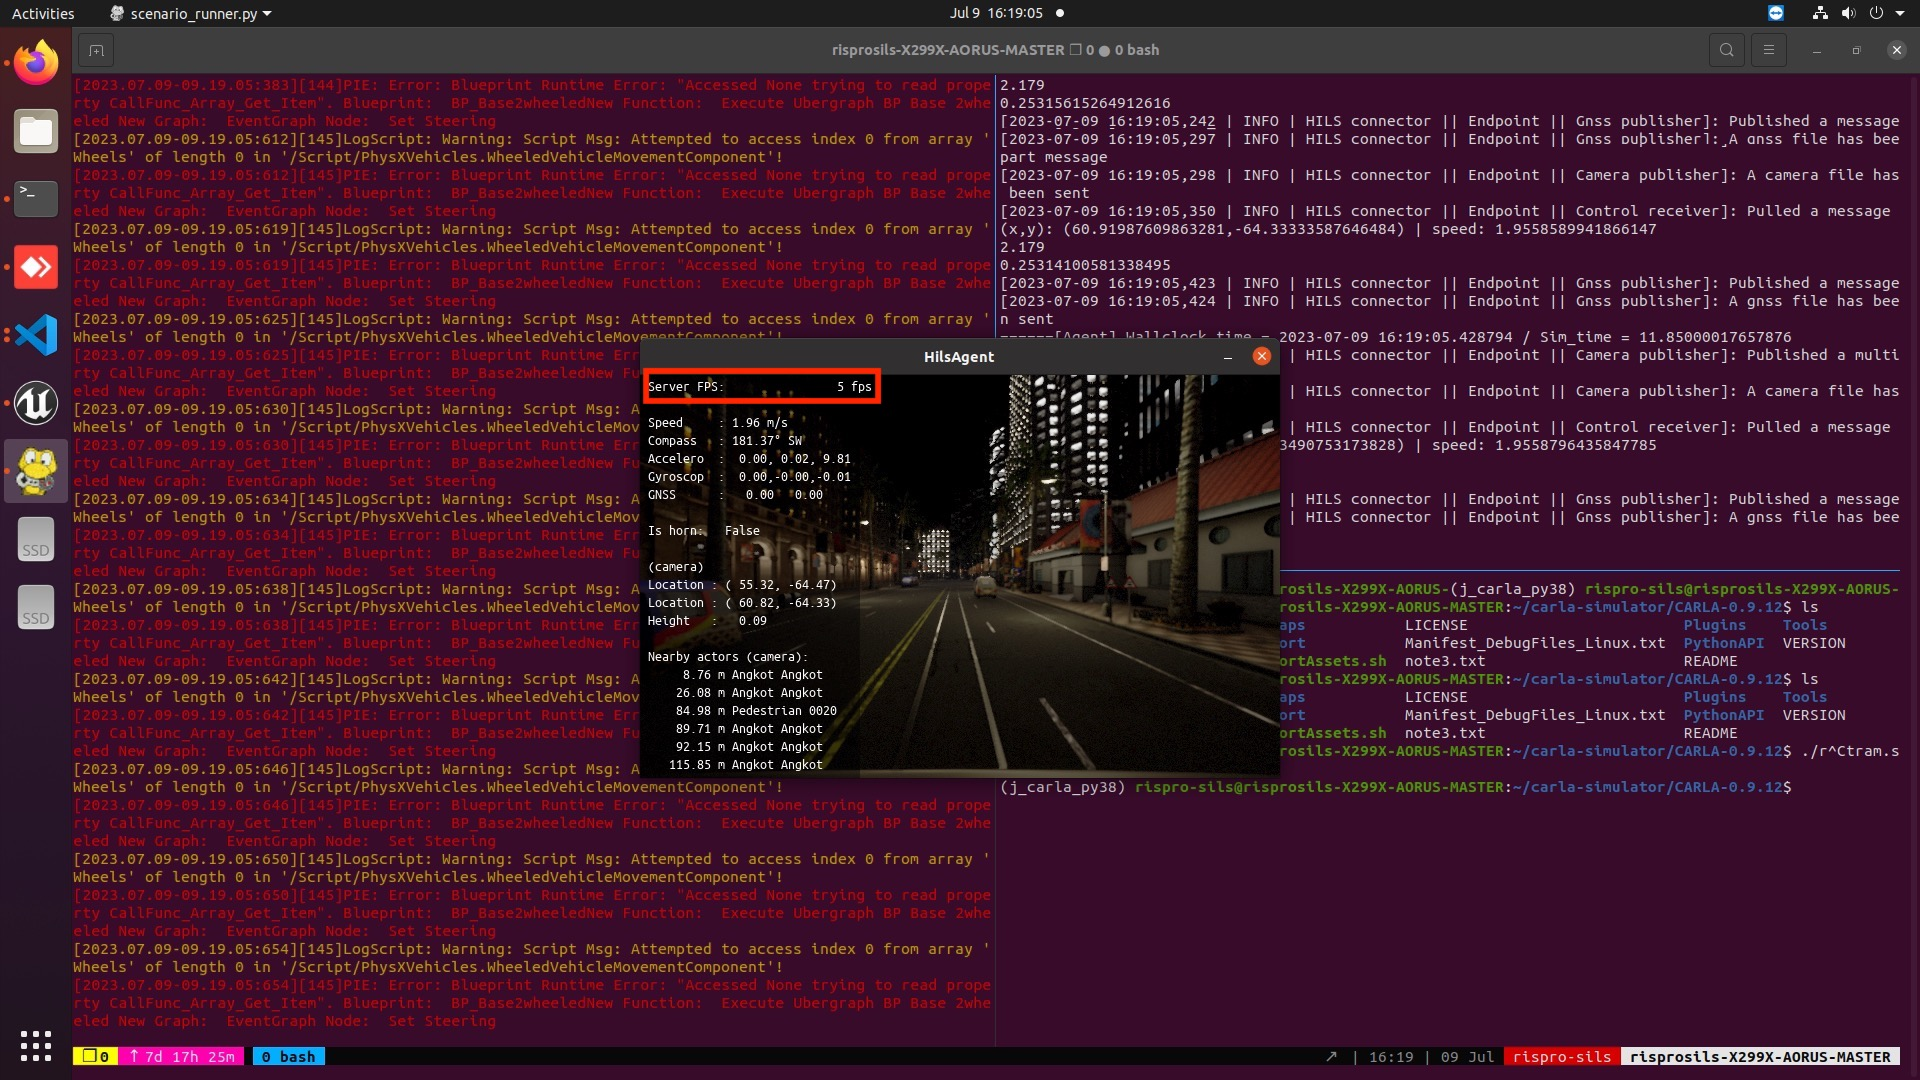
\includegraphics[width=1.0\textwidth,trim={22.5cm 10.5cm 22.5cm 12cm},clip]{resources/chapter-4/CARLA-5FPS.JPG}
	\caption{Bukti CARLA mendapatkan 5 FPS.}
	\label{chapter-4-fig-carla-5-fps}
\end{figure}
\begin{figure}[!htbp]
	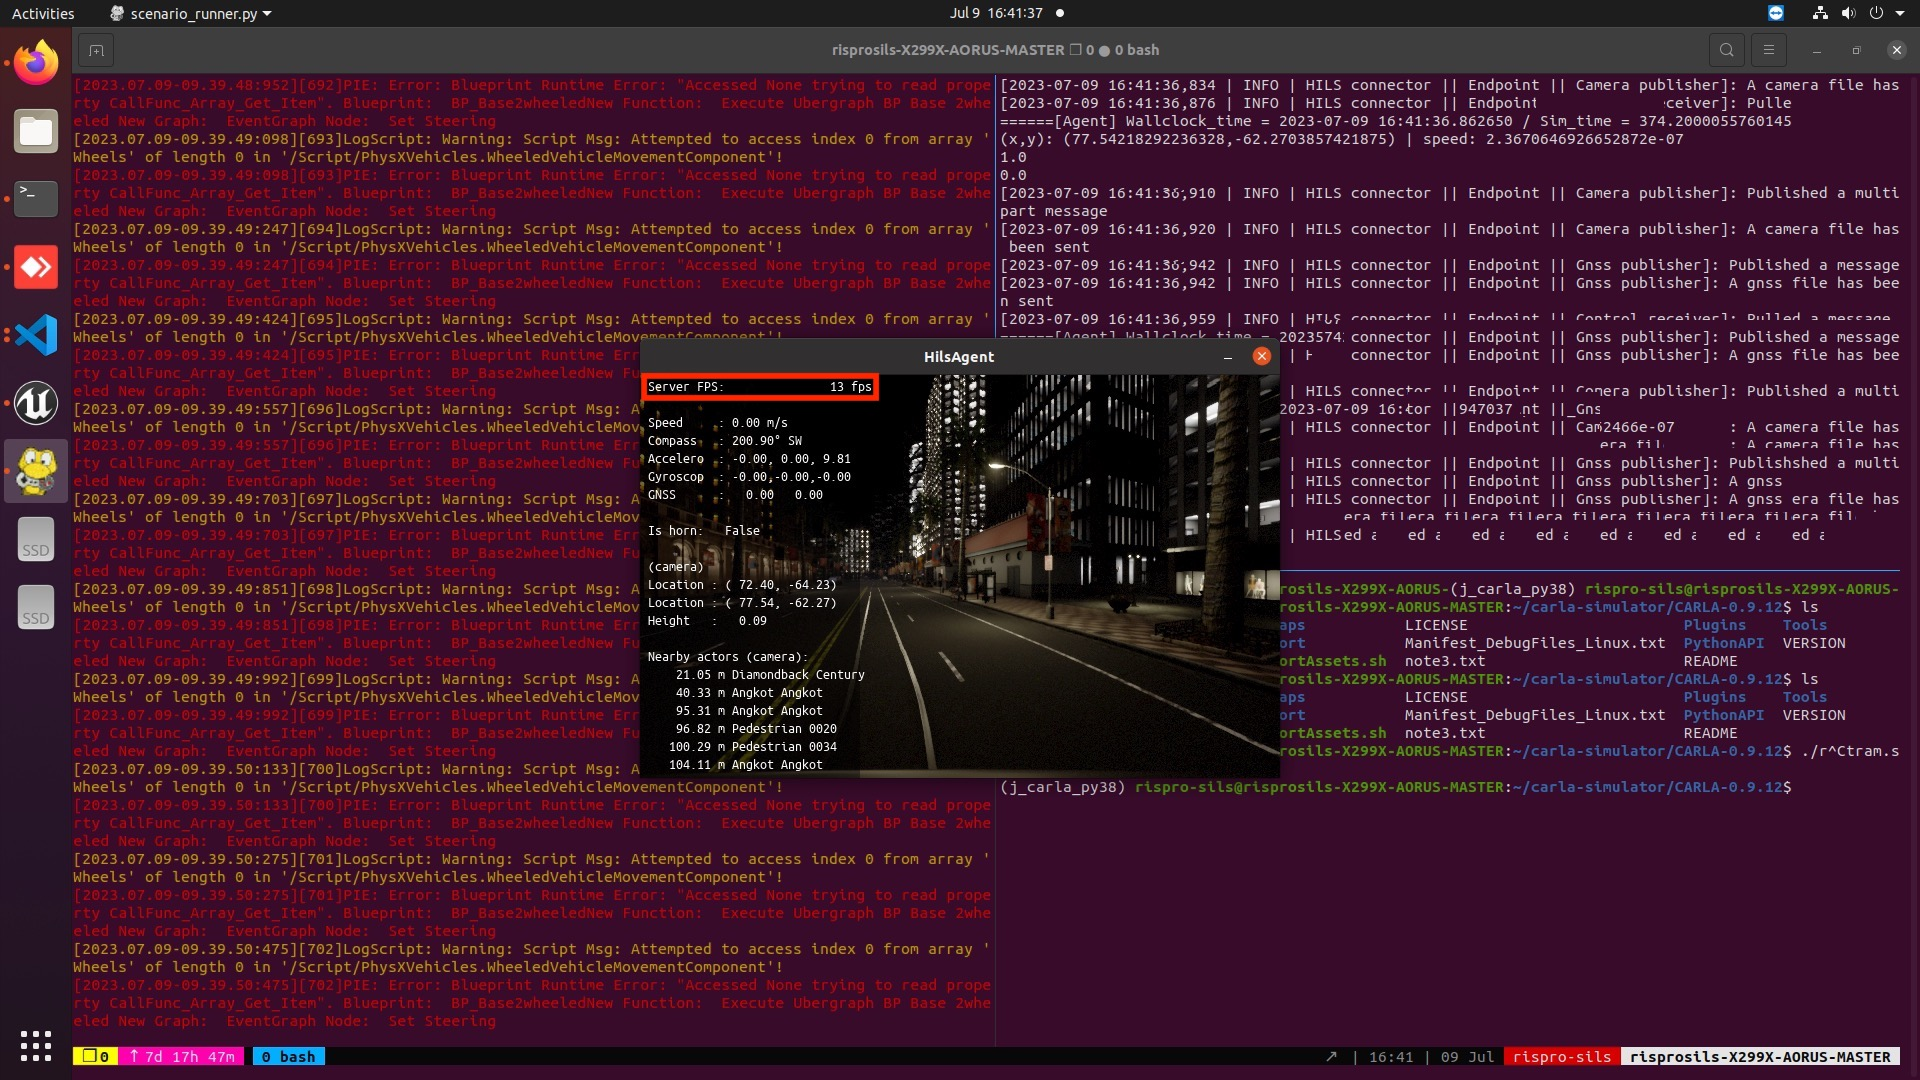
\includegraphics[width=1.0\textwidth,trim={22.5cm 10.5cm 22.5cm 12cm},clip]{resources/chapter-4/CARLA-13FPS.JPG}
	\caption{Bukti CARLA mendapatkan 13 FPS.}
	\label{chapter-4-fig-carla-13-fps}
\end{figure}

Kriteria PERF-02 juga berhasil dilewati. Statistik data dari pengujian dapat
dilihat pada Tabel \ref{chapter-4-tbl-perf-result-statistics}. Selain itu,
persebaran data latensi kedua implementasi mekanisme komunikasi sistem HILS
dapat dilihat pada Gambar \ref{chapter-4-fig-perf-result-old-hils} dan Gambar
\ref{chapter-4-fig-perf-result-new-hils}.
\begin{table}[!htbp]
	\begin{center}
		\begin{tabular}{|l|l|l|}
			\hline
			                   & Jumlah data    & 1.000     \\
			\cline{2-3}
			                   & Rata-rata (ms) & 28,4245   \\
			\cline{2-3}
			                   & Std (ms)       & 4,68      \\
			\cline{2-3}
			\textbf{HILS lama} & Min (ms)       & 16        \\
			\cline{2-3}
			(teoretis)         & $Q_1$ (ms)     & 25        \\
			\cline{2-3}
			                   & $Q_2$ (ms)     & 28        \\
			\cline{2-3}
			                   & $Q_3$ (ms)     & 31        \\
			\cline{2-3}
			                   & Max (ms)       & 45,5      \\
			\cline{2-3}
			\hline

			\hline
			                   & Jumlah data    & 16.891    \\
			\cline{2-3}
			                   & Rata-rata (ms) & 10,989965 \\
			\cline{2-3}
			                   & Std (ms)       & 2,248782  \\
			\cline{2-3}
			\textbf{HILS baru} & Min (ms)       & 4,5       \\
			\cline{2-3}
			                   & $Q_1$ (ms)     & 10        \\
			\cline{2-3}
			                   & $Q_2$ (ms)     & 11        \\
			\cline{2-3}
			                   & $Q_3$ (ms)     & 12,5      \\
			\cline{2-3}
			                   & Max (ms)       & 19,5      \\
			\cline{2-3}
			\hline
		\end{tabular}
	\end{center}

	\caption{Statistik data hasil pengujian kinerja}
	\label{chapter-4-tbl-perf-result-statistics}
\end{table}
\begin{figure}[!htbp]
	\centering
	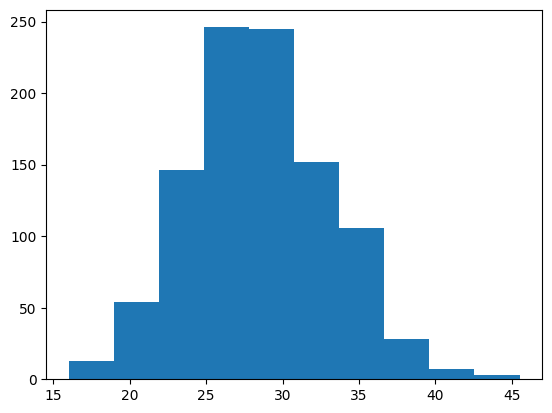
\includegraphics[width=1.0\textwidth]{resources/chapter-4/old-hils-data.png}
	\caption{Persebaran data latensi untuk implementasi teoretis HILS lama}
	\label{chapter-4-fig-perf-result-old-hils}
\end{figure}
\begin{figure}[!htbp]
	\centering
	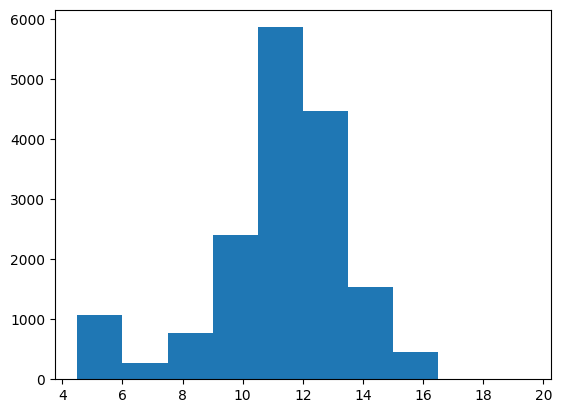
\includegraphics[width=1.0\textwidth]{resources/chapter-4/new-hils-data.png}
	\caption{Persebaran data latensi untuk implementasi HILS baru}
	\label{chapter-4-fig-perf-result-new-hils}
\end{figure}

Ketika menjalankan sistem HILS baru, penggunaan \textit{resource}-nya dapat
dilihat pada Gambar
\ref{chapter-4-fig-perf-result-resource-usage-sils} (komputer SILS) dan Gambar
\ref{chapter-4-fig-perf-result-resource-usage-rkb} (komputer RKB). Selain itu,
Gambar \ref{chapter-4-fig-perf-result-resource-usage-sils-startup} dan
\ref{chapter-4-fig-perf-result-resource-usage-rkb-startup} adalah penggunaan
\textit{Resource} beberapa waktu setelah program dijalankan.
\begin{figure}[!htbp]
	\centering
	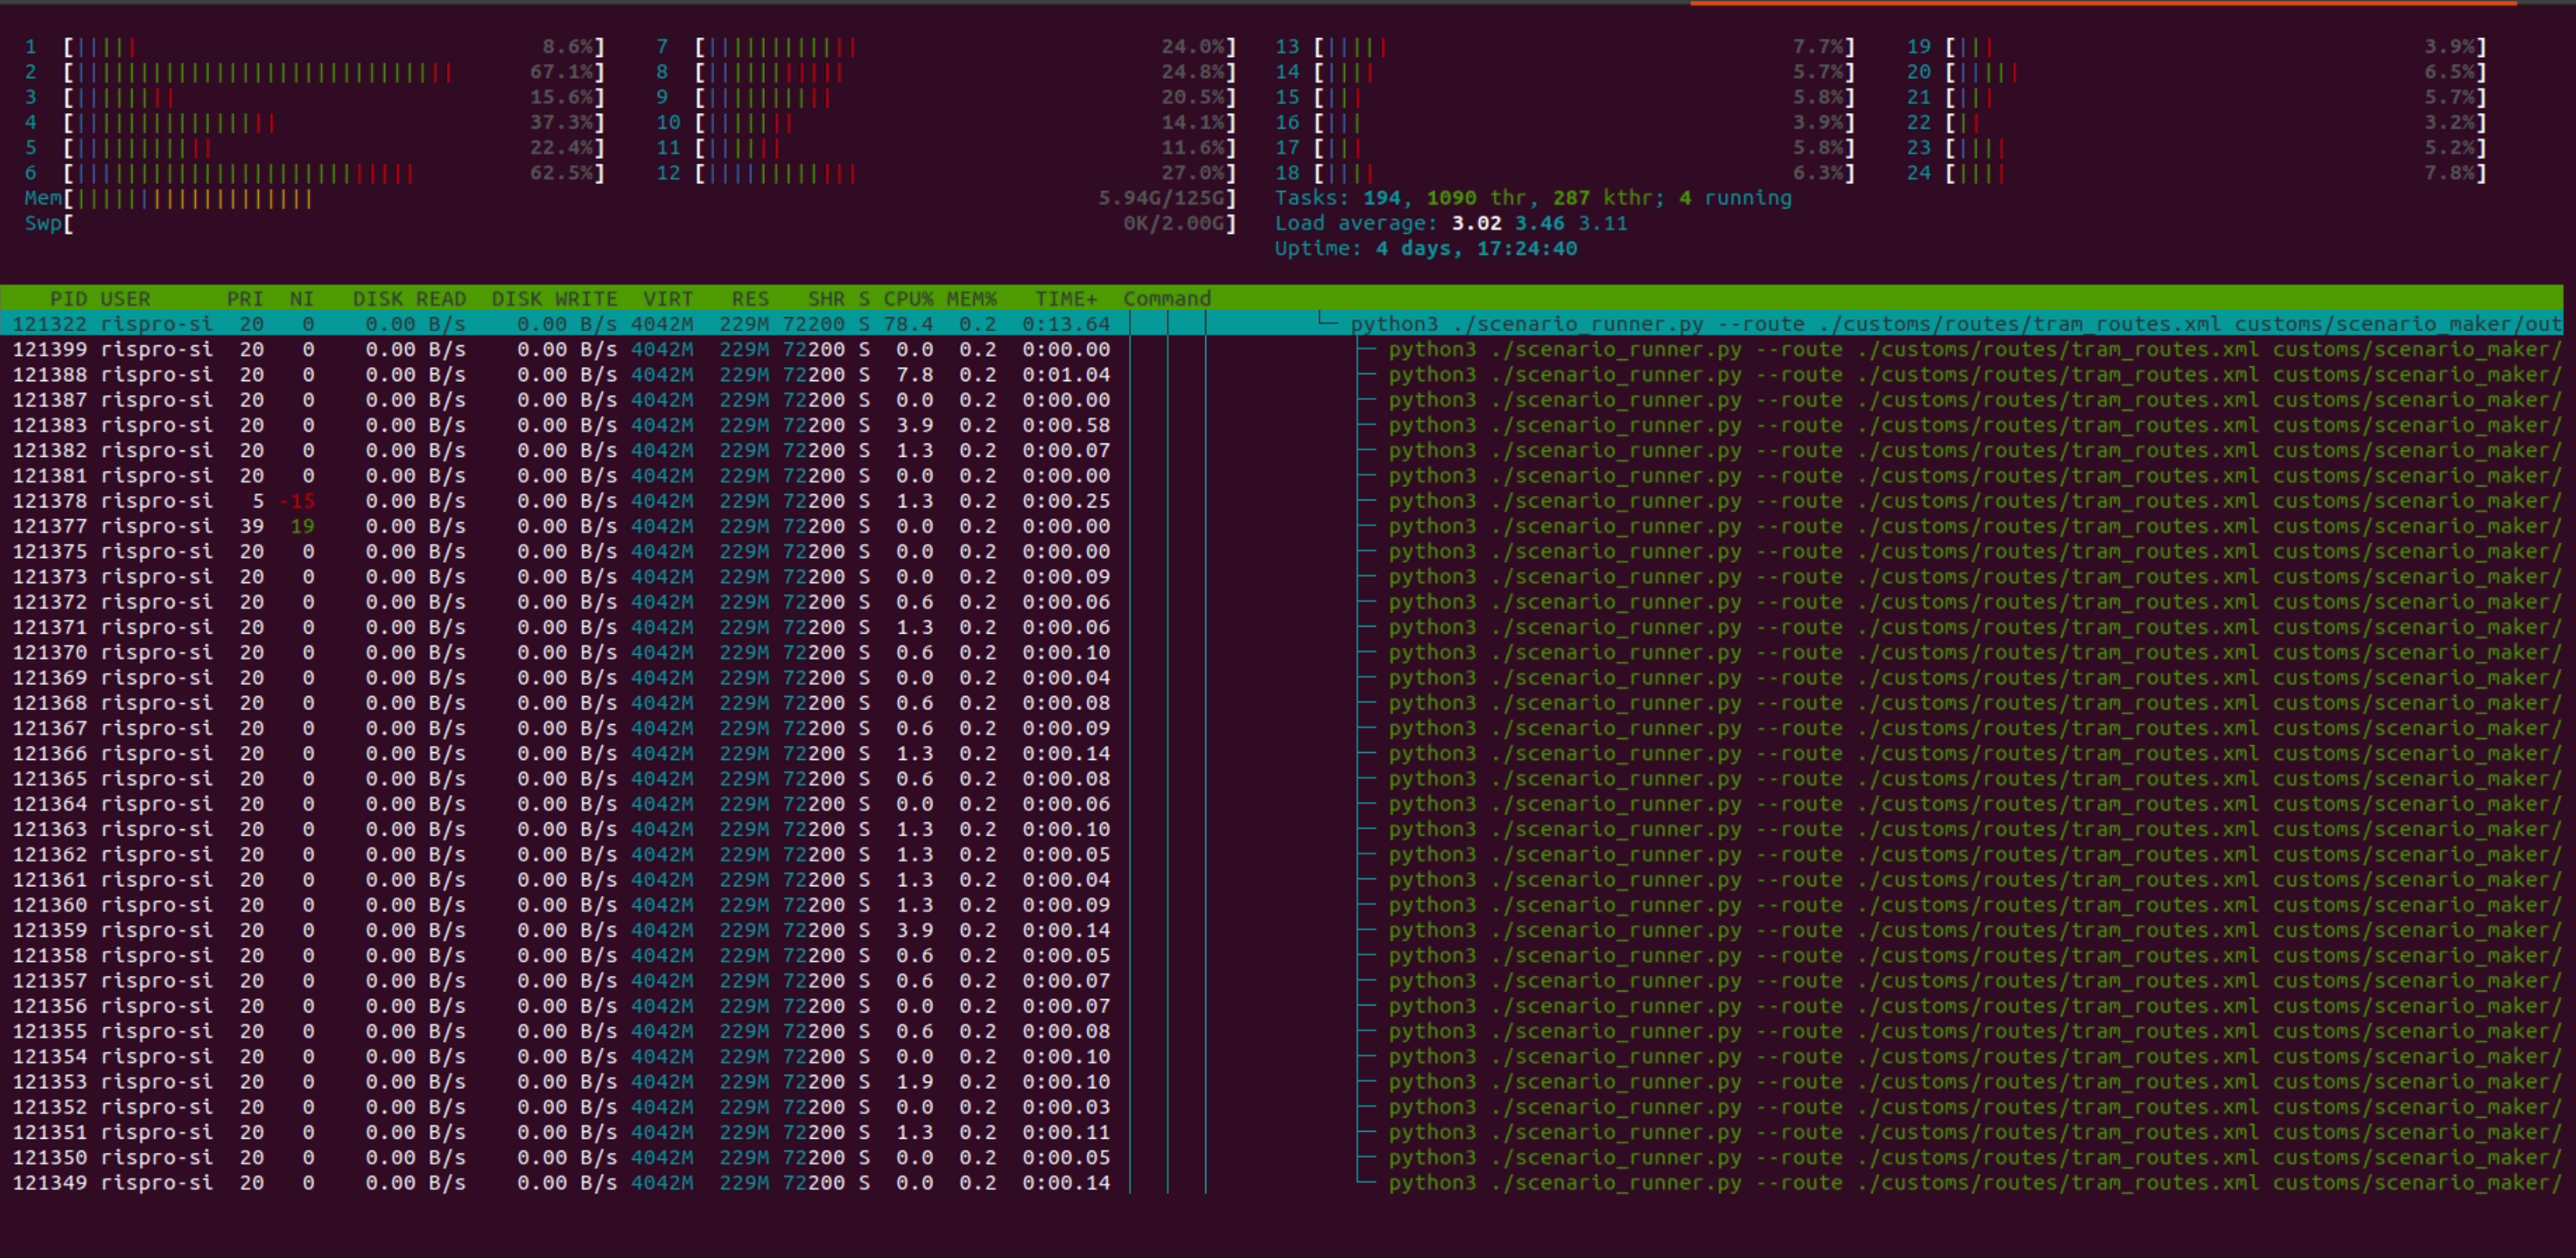
\includegraphics[width=1.0\textwidth]{resources/chapter-4/resource-usage-new-hils-sils-startup.png}
	\caption{Penggunaan \textit{resource} komputer SILS ketika menjalankan sistem HILS baru.}
	\label{chapter-4-fig-perf-result-resource-usage-sils}
\end{figure}
\begin{figure}[!htbp]
	\centering
	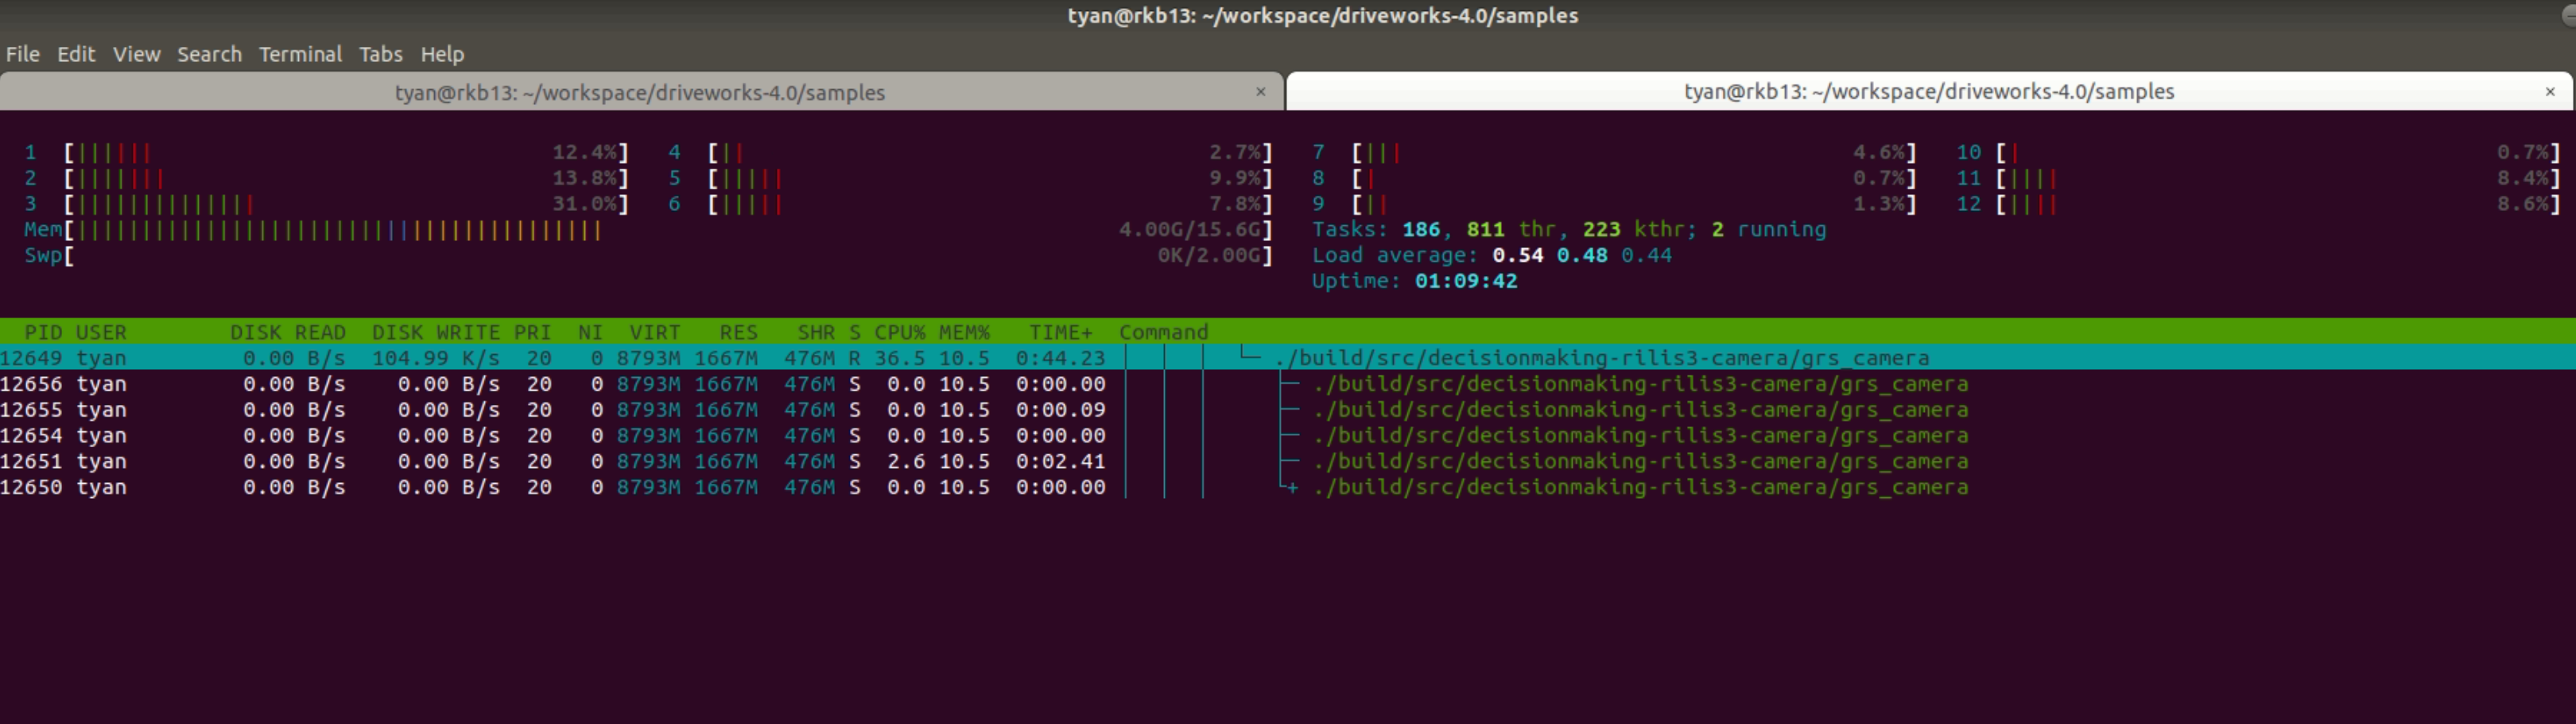
\includegraphics[width=1.0\textwidth,trim={0cm 0cm 0cm 2.5cm},clip]{resources/chapter-4/resource-usage-new-hils-rkb.png}
	\caption{Penggunaan \textit{resource} komputer SILS ketika memulai sistem HILS baru.}
	\label{chapter-4-fig-perf-result-resource-usage-sils-startup}
\end{figure}
\begin{figure}[!htbp]
	\centering
	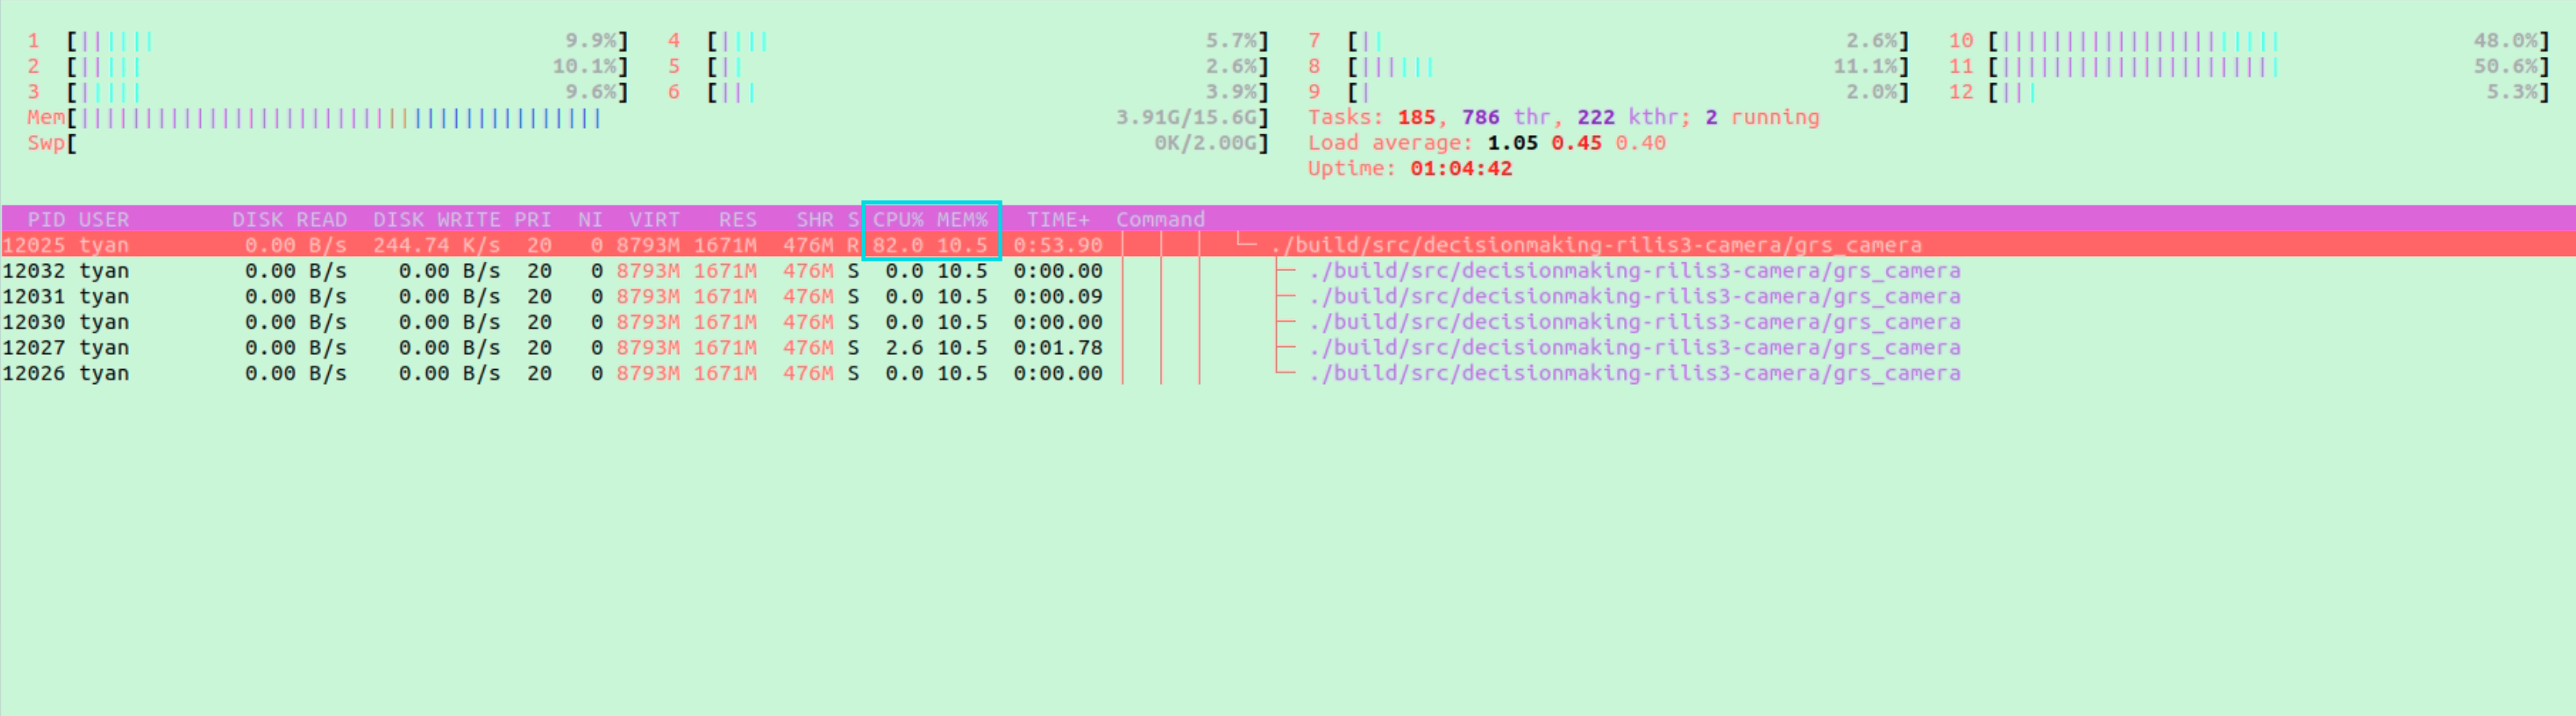
\includegraphics[width=1.0\textwidth]{resources/chapter-4/resource-usage-new-hils-rkb-startup.png}
	\caption{Penggunaan \textit{resource} komputer RKB ketika menjalankan sistem HILS baru.}
	\label{chapter-4-fig-perf-result-resource-usage-rkb}
\end{figure}
\begin{figure}[!htbp]
	\centering
	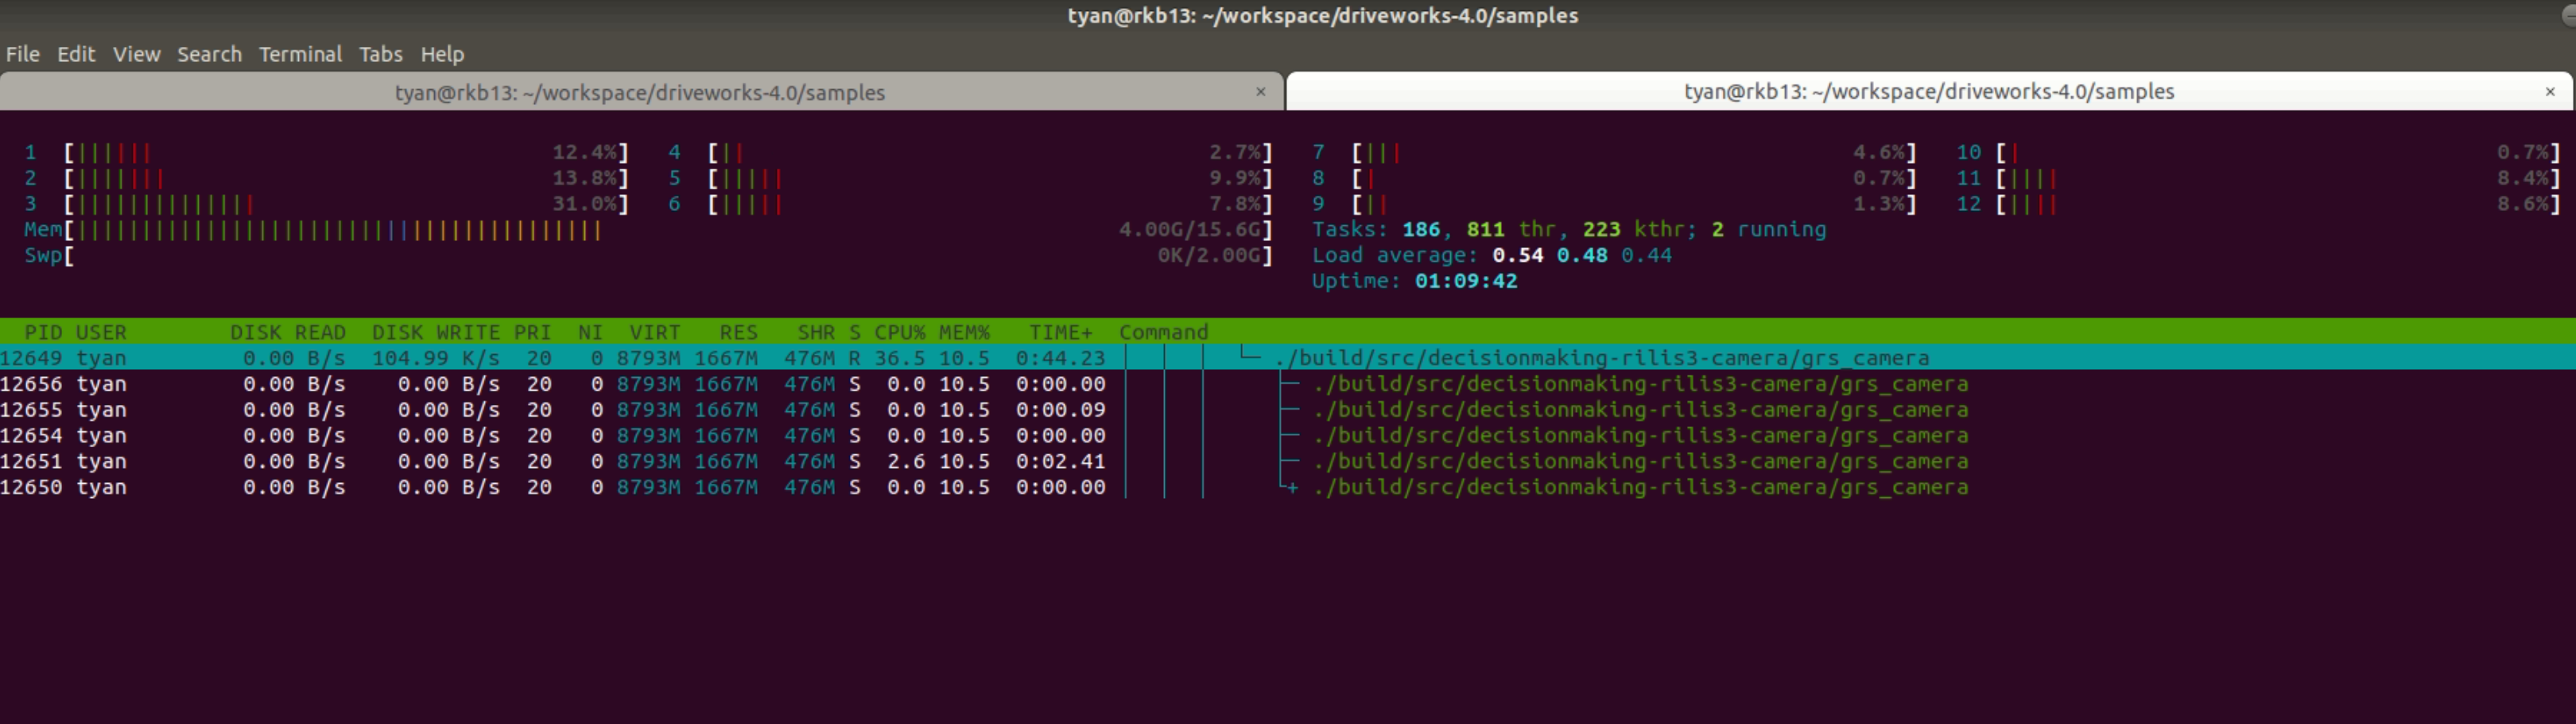
\includegraphics[width=1.0\textwidth,trim={0cm 0cm 0cm 2.5cm},clip]{resources/chapter-4/resource-usage-new-hils-rkb.png}
	\caption{Penggunaan \textit{resource} komputer RKB ketika memulai sistem HILS baru.}
	\label{chapter-4-fig-perf-result-resource-usage-rkb-startup}
\end{figure}

Data lengkap untuk menghitung RTT di pengujian kinerja dapat dilihat pada
Lampiran \ref{appendix-performance-data}. Selain itu, program Jupyter Notebook
yang digunakan untuk pemrosesan data tersebut dapat dilihat pada lampiran
\ref{appendix-algoritma-monitoring}.

\section{Pembahasan Hasil Pengujian}

Dari hasil pengujian dapat dilihat bahwa tujuan pertama dan tujuan kedua tugas
akhir berhasil dicapai. Sistem simulasi yang baru dapat menggunakan data sensor
virtual dari CARLA dan \textit{ego vehicle} pada CARLA dapat dikendalikan
menggunakan kendali dari program GRS. Lalu, pertukaran data sensor dan data
kendali memiliki latensi yang sangat baik. Seperti yang dapat dilihat pada tabel
\ref{chapter-4-tbl-perf-result-statistics}, latensi rata-rata sistem HILS baru
setidaknya 2,5 kali lebih cepat dari sistem HILS sebelumnya. Selain itu,
simulator CARLA juga berhasil berjalan dengan setidaknya 2 FPS.

Meskipun kedua tujuan tugas akhir berhasil dicapai, perlu dicatat bahwa ketika
sensor lidar digunakan kinerja smulator menjadi sangat buruk. Hal ini disebabkan
sensor lidar yang butuh beberapa \textit{step} untuk menghasilkan 1
\textit{frame}. Sensor lidar bekerja dengan berputar sebanyak sepersekian
lingkaran setiap 1 \textit{step}. Sedangkan data dari sensor GNSS dan kamera
hanya butuh 1 \textit{step} untuk menghasilkan 1 \textit{frame} data. Akibatnya
implementasi lidar harus diubah karena ketika pengembangan untuk sensor lidar
diasumsikan sensornya akan seperti sensor kamera, yaitu butuh 1 \textit{frame}.

Selain itu, didapatkan juga bahwa peningkatan kinerja ini dikarenakan perbaikan
pada perangkat lunak, bukan karena perangkat keras. Terlihat penggunaan
\textit{resource} komputer SILS pada gambar
\ref{chapter-4-fig-perf-result-resource-usage-sils} dan komputer RKB pada gambar
\ref{chapter-4-fig-perf-result-resource-usage-rkb} bahwa penggunaan CPU tidak
mencapai 50\% dan penggunaan RAM di sekitar 10\%. Rata-rata penggunaan CPU
berkisar dari 30\%--40\%.

Akan tetapi, dapat dilihat juga pada Gambar
\ref{chapter-4-fig-perf-result-resource-usage-sils-startup} (komputer SILS) dan
Gambar \ref{chapter-4-fig-perf-result-resource-usage-rkb-startup} (komputer RKB)
bahwa ada anomali yang menyebabkan penggunaan CPU melebihi 70\%. Hal ini terjadi
ketika kedua program baru pertama kali dijalankan. Anomali ini mungkin terjadi
karena pada saat \textit{startup}, ada banyak proses yang dilakukan di kedua
program, seperti menyiapkan \textit{window} di GRS dan men-\textit{spawn}
kendaraan serta sensor di ScenarioRunner. Hipotesis itu datang dari fakta bahwa
anomali tersebut hilang setelah terjadi simulasi berjalan dan terjadi pertukaran
data antara kedua komputer/program utama.

\chapter{Penutup}\label{chapter-5}

Pada bab ini akan dijelaskan kesimpulan dari tugas akhir ini serta saran untuk
pengembangan sistem HILS kedepannya dan saran untuk proyek \textit{capstone}.

\section{Kesimpulan}

Dari tugas akhir ini ada beberapa kesimpulan yang dapat dibuat, yaitu
\begin{enumerate}
	\item berhasil dilakukan penulisan ulang mekanisme komunikasi sistem HILS,
	\item sistem HILS yang baru sudah dapat memanfaatkan data sensor virtual
	      dari CARLA serta trem di CARLA berhasil dikendalikan oleh program GRS
	      menggunakan komputer AGX (NVIDIA Pegasus) pada sistem HILS baru, dan,
	\item latensi dan kinerja pada sistem HILS dengan mekanisme komunikasi baru
	      setidaknya secara rata-rata 2,5 kali lebih cepat jika dibandingkan
	      dengan sistem HILS sebelumnya.
\end{enumerate}

\section{Saran}

Saran untuk pengembangan sistem HILS adalah sebagai berikut.
\begin{enumerate}
	\item perbaikan kode pustaka agar dapat menggunakan sensor lidar virtual,
	\item pengujian dengan multi-kamera untuk menguji sistem dapat menggunakan
	      agar lebih sesuai dengan dunia nyata,
	\item pengujian dengan berbagai mekanisme/protokol komunikasi lain untuk
	      mencoba mengurangi \textit{overhead} kinerja akibat jaringan, dan
	\item mengurangi jumlah kelas yang berinteraksi langsung dengan program
	      ScenarioRunner dari empat menjadi satu kelas.
	      % \item membuat penerimaan data di sisi program GRS terjadi secara paralel.
\end{enumerate}

Berikut adalah saran untuk proyek \textit{capstone} pengembangan trem.
\begin{enumerate}
	\item memperbaiki kode program GRS karena sangat sulit untuk dibaca dan
	      dimodifikasi, dan
	\item menambahkan \textit{code review}, \textit{static code analysis}, dan
	      Git \textit{flow} untuk program GRS untuk menjaga kualitas dan keamanan
	      kode.
\end{enumerate}

%----------------------------------------------------------------%

% Daftar pustaka
\printbibliography

% Setting judul lampiran
\titlespacing*{\chapter}{0pt}{0pt}{0pt}
\titlespacing*{\section}{0pt}{0pt}{*1}

% Setting judul anak lampiran
\titleformat*{\section}{\bfseries}

% Index
\appendix
\chapter{Arsitektur Baru Sistem Simulasi}\label{appendix-arsitektur-baru}
\begin{figure}[ht]
	\begin{center}
		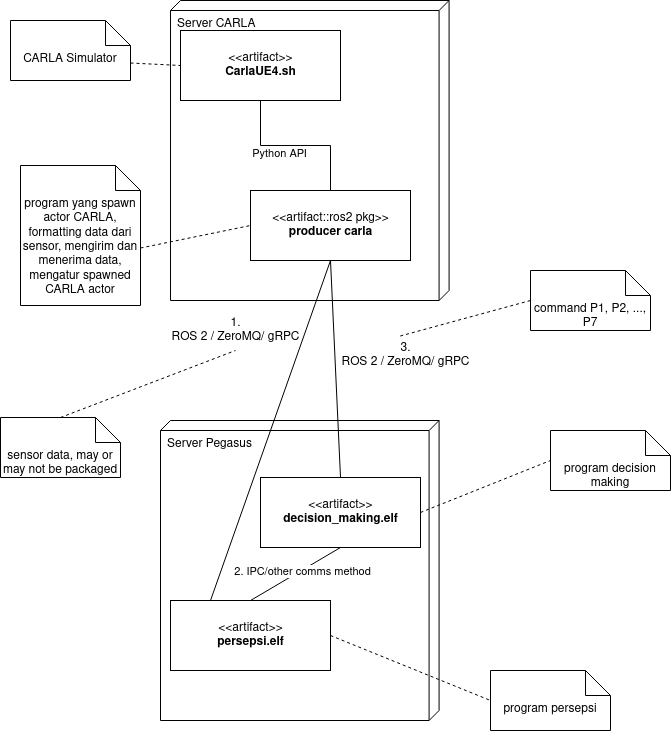
\includegraphics[width=1.0\textwidth]{resources/appendix-1-deployment diagram.png}
		\caption{Arsitektur Baru untuk Sistem Simulasi}
	\end{center}
\end{figure}
% TODO: find a better way to set counter
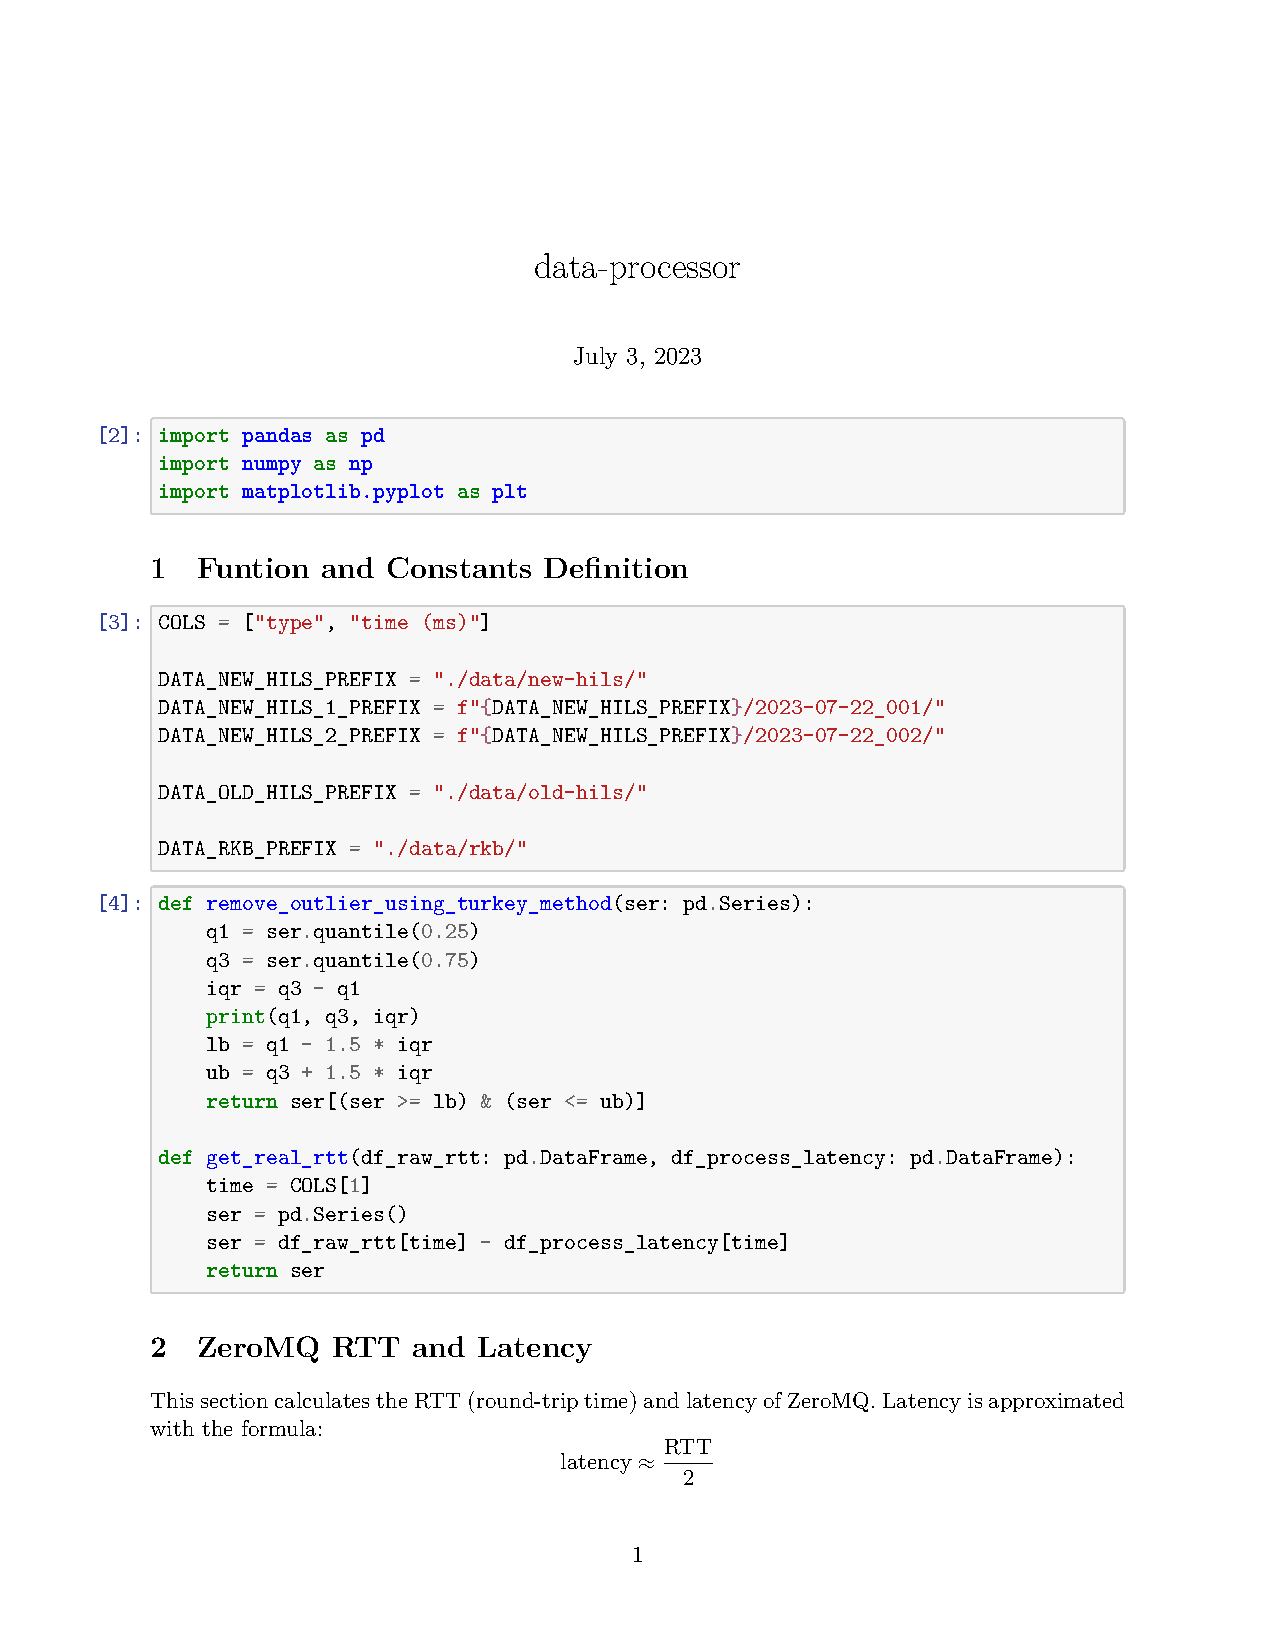
\includepdf[pages=1,scale=.7,pagecommand={\chapter{Program Pemrosesan
Data}\label{appendix-algoritma-monitoring}\setcounter{section}{0}},linktodoc=true]{resources/appendix-2-data-processor.pdf}
\includepdf[pages=2-,scale=.7,pagecommand={},linktodoc=true]{resources/appendix-2-data-processor.pdf}

\chapter{Rencana Umum Proyek}
% TODO: find a better way to set counter
\setcounter{section}{1}


\end{document}
